\chapter{Further Experiments on Basic Colour Systems}
\label{s:basic-experiments}

Once all the operators have been provided for a particular language
strategy, various in-depth studies on various aspects of language
systems based on that language strategy are possible. In this chapter,
I will study language systems that are based on the basic colour
strategy. First, I will study the impact of colour distributions in
the environment of the agents on the similarity between individually
learned colour systems and human colour systems in Section
\ref{s:impact-of-environment} \citep{belpaeme09impact}. Next, I will
investigate the impact of language on the similarity between universal
trends that have been reported in literature in Section
\ref{s:impact-of-language} and colour systems that result from
simulation \citep{belpaeme05eelc, belpaeme05explaining,
  belpaeme07language}. Both these experiments have been conducted in
collaboration with Tony Belpaeme. Finally, I will examine the impact
of embodiment on the performance of the adoption, alignment and
invention operators of the \emph{basic colour strategy} in Section
\ref{s:experiments-grounded} \citep{bleys09grounded}.

\section{Impact of environment on similarity to natural systems}
\label{s:impact-of-environment}
\is{impact!of environment on basic colour systems}

Ever since \cite{berlin69basic} observed that colour categories show a
remarkable cross-cultural similarity, there has been an
ongoing debate on what the main cause of this universal character of
colour categories might be. Some authors
\citep{vanwijk59crosscultural, shepard92perceptual,
  yendrikhovskij01computational} claim that this cross-cultural
similarity is due to the shared environment in which individuals use
their colour categories. These environments exhibit statistical
distributions by which colours occur, which are not uniform. It is
claimed that these distributions limit the number of possible
configurations of the colour category systems.

\cite{yendrikhovskij01computational} presented computational
simulations that support this view. He demonstrated how the
distribution of colours in natural images can be used to extract
colour categories that resemble human colour categories. For this
purpose, the colour information of 10k pixels drawn from images of
natural scenes was converted to a perceptual colour space (CIE
$L^*u^*v^*$) and an unsupervised clustering algorithm was used to
extract a number of
clusters. \citeauthor{yendrikhovskij01computational} showed how these
clusters resemble the colour categories of American subjects
\citep{boynton87locating}. This was shown by matching the cluster
centroids to the English colour categories and computing the
correlations between each dimension of the CIE $L^*u^*v^*$ colour
space, the chroma $C^*_{uv}$ and the hue $h^*_{uv}$. The correlations
were high, ranging from $r = 0.762$ for lightness to $r = 0.999$ for
hue.

Without denying the importance of
\citeauthor{yendrikhovskij01computational}'s work, we would like to
critically assess the evidence and extend his work. In order to truly
validate the claim that the high correlations to human colour
categories are mainly due to the colour distributions in the
environment, it is essential to compare the reported results starting
from a control dataset in which no such distribution is present
(i.e. each colour occurs with the same probability). Only if the
correlations between the centroids found in the latter dataset is
significantly lower than those originally reported, one can conclude
that the high correlation in the original study is due to the colour
distribution present in the original dataset. In order to measure the
importance of the colour distribution, one could also start from a
different set of pictures and compare the results to those reported in
the original study.

\subsection{Data sets}
\label{s:simulated-data-sets}

Two sets of photographs have been collected, one containing natural
images and the other urban images. The nature collection was compiled
from image databases on the internet, and contains imagery of animals,
flowering plants and landscapes. The urban collection contains
photographs shot with a digital camera (Olympus C-4000 ZOOM) in a
Northern European environment; it contains imagery of buildings,
people and urban activities, both indoor and outdoor; both collections
contain 300 images.

From both image sets 25k RGB-pixels were randomly selected, one which
I will call the \emph{natural data set} and the other which I will
indicate as the \emph{urban data set}. I also added a control dataset,
called \emph{uniform data set} which consists of 25k random RGB
values, to test the null-hypothesis that categories are not influenced
by the chromatic distribution in the environment. All RGB values have
been converted to both the CIE $L^*a^*b^*$ and CIE $L^*u^*v^*$ colour
space. A projection of the three data sets on the $a^*b^*$ plane are
shown in Figure \ref{f:simulated-data-sets}.

A first analysis of the data reveals that natural and urban data sets
indeed contain a non-random structure. Figure
\ref{f:data-sets-histogram} shows histograms of the CIE $L^*a^*b^*$
values of the data sets. While the uniform data set has a quasi
uniform distribution, the natural and urban data sets have a higher
distribution of lowly saturated colours. This confirms previous
observations of the chromatic content of natural scenes
\citep{howard94colors} that natural occurring
colours occupy a restricted area of the chromaticity diagram.

\begin{figure}[htbp]
\centering
\subfigure[]{
    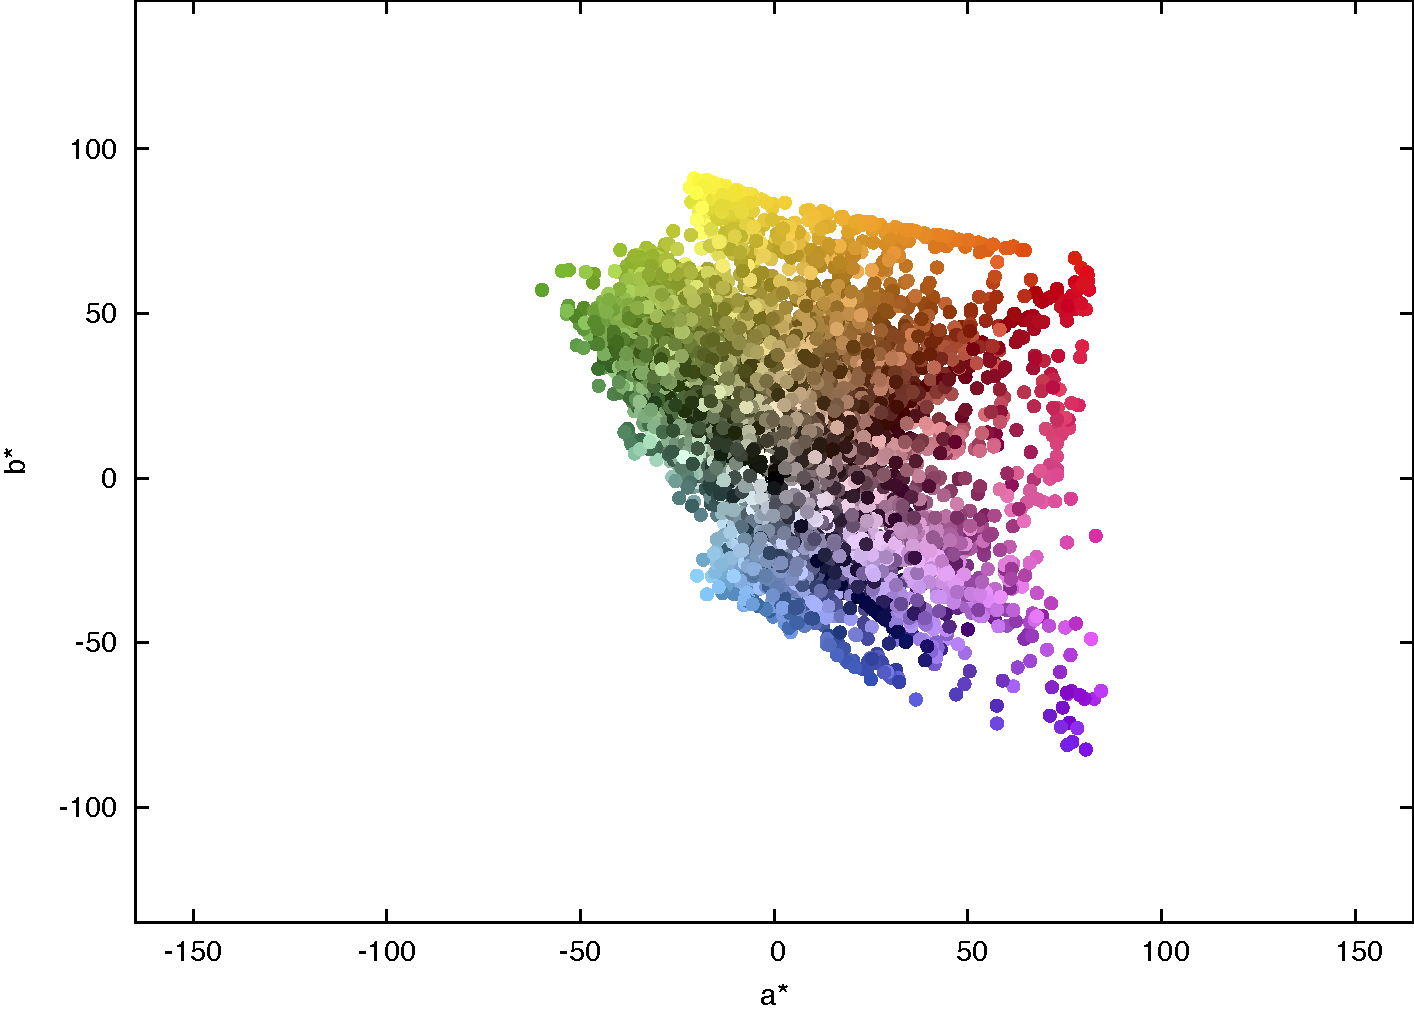
\includegraphics[width=.47\textwidth]{./experiments/figures/natural-data-set.pdf}
  \label{f:natural-data-set}
}
\subfigure[]{
    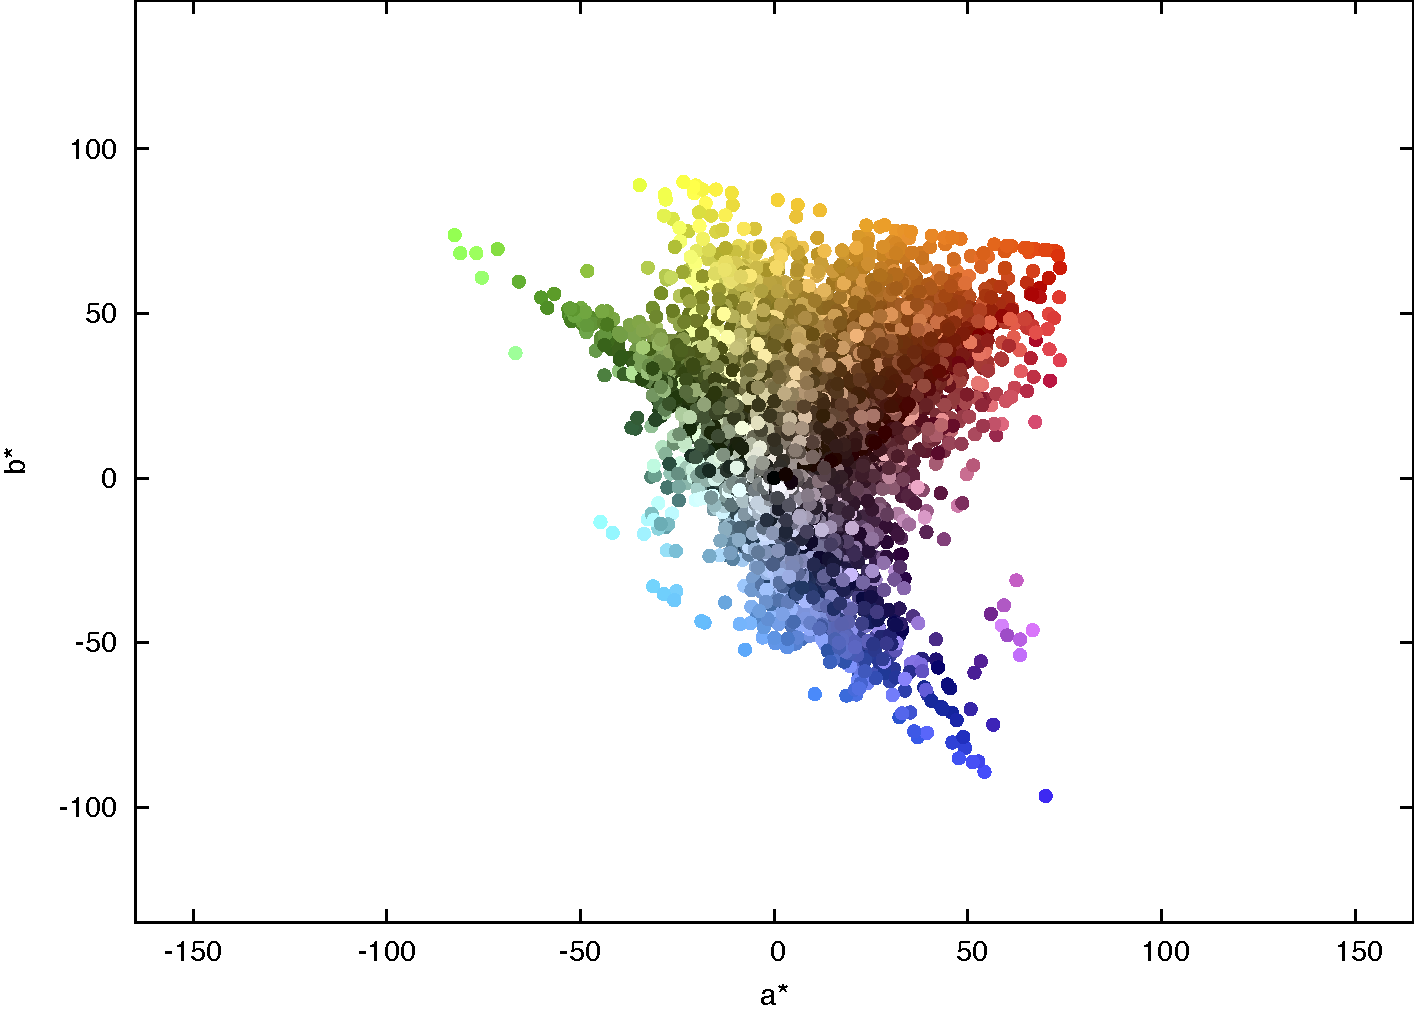
\includegraphics[width=.47\textwidth]{./experiments/figures/urban-data-set.pdf}
  \label{f:urban-data-set}
}
\subfigure[]{
    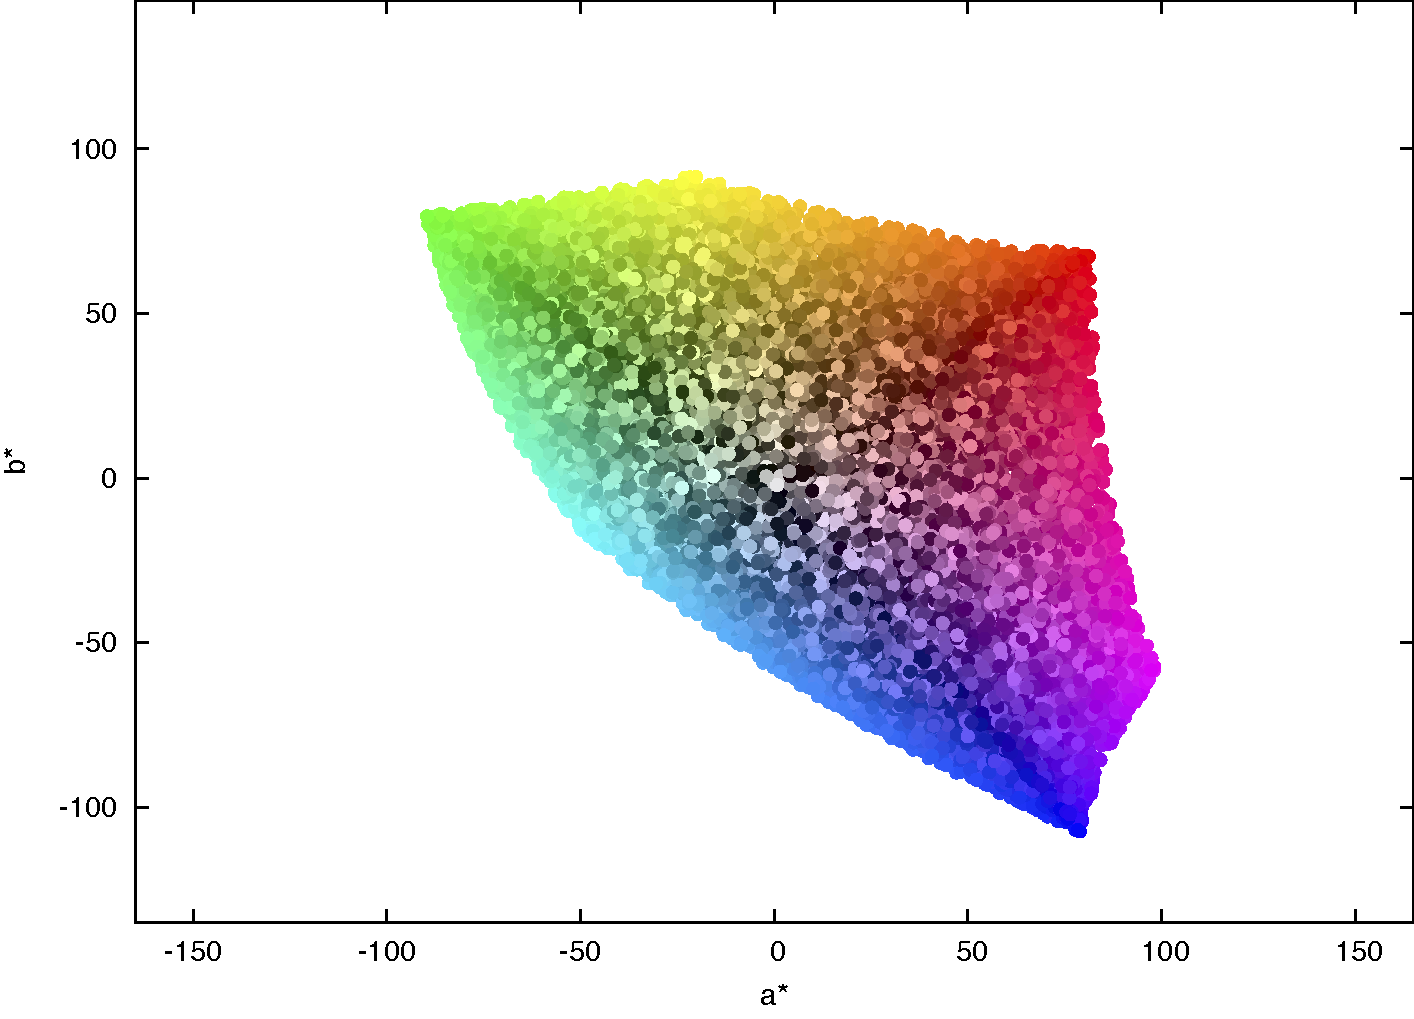
\includegraphics[width=.47\textwidth]{./experiments/figures/uniform-data-set.pdf}
  \label{f:uniform-data-set}
}
\caption[Three different simulated data sets]{Three different
  simulated data sets, projected on the $a^*b^*$ hue plane of the CIE
  $L^*a^*b^*$ colour space: \subref{f:natural-data-set} the natural
  data set; \subref{f:urban-data-set} the urban data set;
  \subref{f:uniform-data-set} the uniform data set}
\label{f:simulated-data-sets}
\end{figure}

\begin{figure}[htbp]
\centering
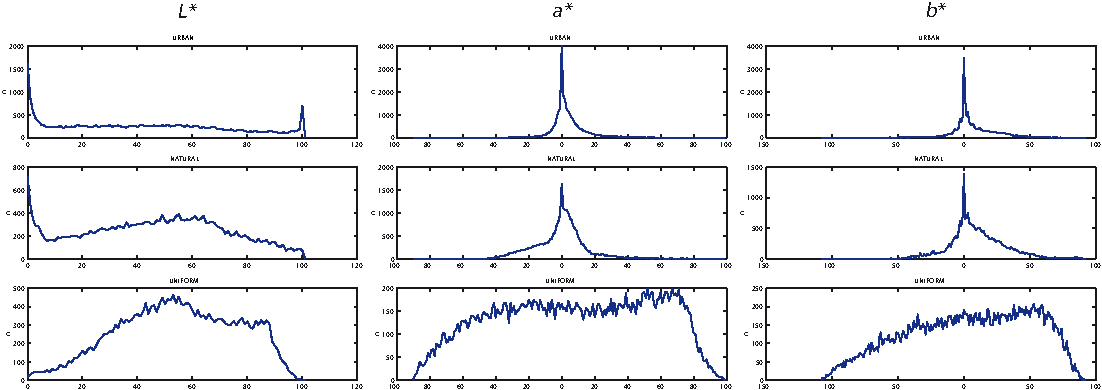
\includegraphics[width=\textwidth]{./experiments/figures/data-sets-histogram.pdf}
\caption[Histogram of three different simulated data sets per
channel]{Histogram of the three different simulated data sets per
  channel. The urban and natural data set contain more unsaturated
  colours than the uniform data set.}
\label{f:data-sets-histogram}
\end{figure}

\subsection{Extracting colour categories}

As clustering algorithm I used the $k$-means clustering algorithm
\citep{lloyd82least}. $k$-means clustering uses an iterative
re-estimation procedure. Initially, $k$ data points are selected as
initial centroids. All data points are assigned to the nearest
centroid (according to the distance between the sample and the
centroid). The centroids are recalculated to be the mean of all the
samples that are associated to it.  After the recalculation all the
samples are classified again and the centroids are recomputed. This
algorithm continues until a stop criterion is met, usually when there
is no further change in the assignment of the data points.

As $k$-means clustering is not deterministic (a random seed is needed
to select the initial centroids), the clusters found by each run of
the algorithm might vary. How much the clusters vary depends on the
structure of the data. To deal with possible variation in the found
clusters, the colour data was clustered $1000$ times. The variation in
the outcome of the centroids found by the algorithm for the datasets I
am using, is illustrated in Figure \ref{f:clustering-first}. The $1000
\times k$ centroids are then clustered again using $k$-means
clustering, but now the initial points are each time chosen to be
equal to the outcome of one run in the previous phase. From these
solutions, the one in which the average distance between the $1000
\times k$ centroids and the nearest centroid in the solution is
minimal, is chosen to be the final $k$ clusters. The goal of this
additional step is to avoid some algorithm specific problems due to
outliers in the original dataset \citep{bradley98refining}.

\begin{figure}[htbp]
\centering
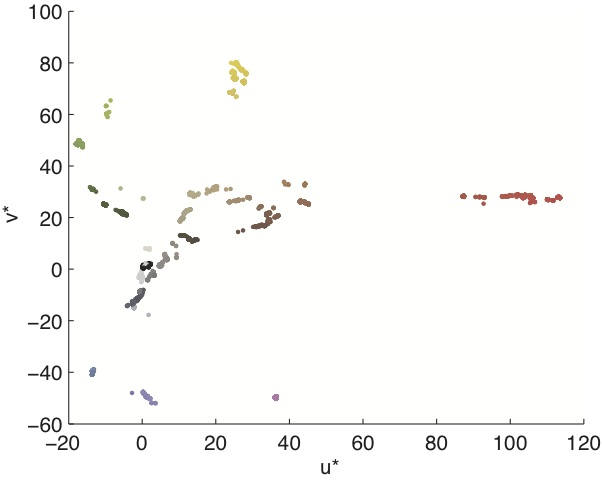
\includegraphics[width=.7\textwidth]{./experiments/figures/clustering-first.jpg}
\caption[Example of the variation of the centroids found by the
k-means clustering algorithm]{Typical example of the variation of the
  centroids found after running the standard k-means clustering
  algorithm. The collection of the centroids of 1000 independent runs
  of the algorithm is projected on the $u^*v^*$-plane for the natural
  data-set for k = 11.}
\label{f:clustering-first}
\end{figure}

\subsection{Comparison to human colour categories}

To compare the impact of the statistical distribution on the resulting
centroids several analyses can be performed. I provide the results of
two such analyses.

The first analysis is based on a correlation measure (Kendall's Tau)
for each dimension. This non-parametric test does not require data to
have a certain distribution \citep{conover99practical}. The test
returns values between $-1$ and 1. A value of 1 indicates that the
correlation is complete and $-1$ that the correlation is complete, but
inverse. A value of 0 indicates that no linear correlation could be
found, while values closer to 1 or $-1$ indicate an increasing
correlation. The correlation was computed for 11 clusters. Table
\ref{t:clustering-correlation} reports the correlations between the
centroids extracted from the natural, urban and uniform data sets and
the English categories, both for CIE $L^*a^*b^*$ and CIE $L^*u^*v^*$.

\begin{table}[htbp]
\centering
\begin{tabular}{>{\scshape}ld{5}d{5}d{5}d{5}d{5}}
\lsptoprule
& \multicolumn{1}{c}{$L^*$} & \multicolumn{1}{c}{$u^*$} & \multicolumn{1}{c}{$v^*$} & \multicolumn{1}{c}{$C^*_{uv}$} & \multicolumn{1}{c}{$H_{uv}$}\\
\midrule
natural & 0.561^*  & 0.673^*  & 0.636^*  & 0.709^*  & 0.745^*  \\
urban & 0.972^*  & 0.564^*  & 0.673^*  & 0.636^*  & 0.636^*  \\
uniform & 0.187  & 0.418  & 0.745^*  & 0.491^*  & 0.818^*  \\
\midrule
& \multicolumn{1}{c}{$L^*$} & \multicolumn{1}{c}{$a^*$} & \multicolumn{1}{c}{$b^*$} & \multicolumn{1}{c}{$C^*_{ab}$} & \multicolumn{1}{c}{$H_{ab}$}\\
\midrule
natural & 0.785^* & 0.200 & 0.745^{*} & 0.709^* & 0.636^* \\
urban & 0.935^{*} & 0.382 & 0.745^{*} & 0.491^* & 0.345 \\
random & 0.411 & 0.309 & 0.782^{*} & 0.600^* & 0.709^* \\
\lspbottomrule
\multicolumn{6}{l}{\footnotesize* Correlation is significant at the 0.05 level.}\\	
\end{tabular}
\caption{Correlation between cluster centroids and human colour
  categories in the CIE $L^*a^*b^*$ and CIE $L^*u^*v^*$ colour space.}
\label{t:clustering-correlation}
\end{table}

The high correlations between the centroids extracted from the natural
and urban data sets and the English colour categories
\citep{sturges95location} confirm the results of
\citeauthor{yendrikhovskij01computational}. However, the correlation
remains high (although somewhat lower) for the uniform dataset. As the
uniform data set contains no chromatic structure, as opposed to the
natural or urban data sets, one would expect the correlation for this
set to be zero on average. Nevertheless, the uniform data set still
results in clusters having a remarkably positive correlation with
human colour categories, which allows me to reject the explanation
offered by \citeauthor{yendrikhovskij01computational}. This can only
be explained by the structure of the colour space and the nature of
the clustering algorithm.

For the second analysis, I created a benchmark test to compare the
performance of each resulting set of centroids in more detail. This
benchmark consists of naming one hundred consensus chips (i.e. chips
for which there was unanimous agreement in colour naming) of the study
of \citeauthor{sturges95location} (shown in Figure
\ref{f:basic-consensus-chips-english}). In order to name these chips,
a matching process is required to associate each centroid to one of
the English colour categories. Each consensus chip is named using the
colour term of the associated English colour category, using a
nearest neighbour algorithm based on the centroids. The results,
broken down by each category, are summarised in Table
\ref{t:clustering-benchmark}.

\begin{table}[htbp]
  \centering
  \footnotesize
  \begin{tabular}{>{\scshape}crrrrrrrrrrrr}
    \lsptoprule
    & \multicolumn{1}{c}{WE} & \multicolumn{1}{c}{GY} & \multicolumn{1}{c}{BK} & \multicolumn{1}{c}{GN} & \multicolumn{1}{c}{YW} & \multicolumn{1}{c}{BL} & \multicolumn{1}{c}{RD} & \multicolumn{1}{c}{PU} & \multicolumn{1}{c}{BR} & \multicolumn{1}{c}{OR} & \multicolumn{1}{c}{PK} & \multicolumn{1}{c}{\scshape total}\\
    & 2 & 6 & 3 &22 & 8 & 25 & 4 & 14 & 4 & 6 & 6 & 100 \\
    \midrule
    s\&w & 2 & 6 & 3 & 17 & 8 & 18 & 4 & 9 & 4 & 6 & 6 & 83\\
    nat & 2 & 1 & 3 & 8 & 8 & 11 & 4 & 6 & 2 & 0 & 0 & 45 \\
    urb & 2 & 4 & 2 & 5 & 8 & 18 & 4 & 2 & 0 & 0 & 3 & 48 \\
    uni & 2 & 0 & 3 & 2 & 0 & 5 & 4 & 0 & 0 & 1 & 3 & 20 \\
    \midrule
    s\&w & 2 & 6 & 3 & 18 & 8 & 18 & 4 & 9 & 4 & 6 & 6 & 84 \\
    nat & 2 & 5 & 3 & 15 & 8 & 24 & 4 & 6 & 0 & 0 & 1 & 68 \\
    urb & 2 & 5 & 3 & 5 & 8 & 24 & 4 & 6 & 2 & 0 & 2 & 61 \\
    uni & 2 & 0 & 3 & 13 & 8 & 0 & 4 & 1 & 0 & 4 & 4 & 39 \\
    \lspbottomrule
  \end{tabular}
  \normalsize
  \caption[Naming benchmark for cluster centroids]{Number of correctly
    named consensus samples broken down by category: white (WE), grey
    (GY), black (BK), green (GN), yellow (YW), blue (BL), red (RD),
    purple (PU), brown (BR), orange (OR) and pink (PK). The total
    number of consensus chips is shown on top. The top part represents
    the results in CIE $L^*a^*b^*$, the bottom part in CIE
    $L^*u^*v^*$. The results are shown for the categories found in
    English (S\&W) and all three datasets: natural (NAT), urban (URB)
    and uniform (UNI). Only the results for 11 centroids are shown.}
  \label{t:clustering-benchmark}
\end{table}

A first important observation from these results is that even when
the English categories of the same study are used, the benchmark only
reaches about 83\% of success. This suggests that, although capable of
accounting for more than three quarters of the consensus chips, the
one-nearest neighbour classification algorithm might be too general to
capture all the richness of human colour categories. This first result
sets the maximal level of success one might hope to achieve when using
this particular classification algorithm.

The performance of the centroids resulting from the uniform data set
is still quite good (from a quarter to a half of the maximal expected
performance, depending on the used colour space). This can only be
accounted for by the shape of the colour spaces and the clustering
algorithm that were used but not by any statistical distribution in
the environment. However, if such a distribution is present in a data
set, such as in the natural and urban data sets, it significantly
improves the performance of the benchmark by about a third of the
maximal expected performance. When using the CIE $L^*a^*b^*$ or CIE
$L^*u^*v^*$ colour space, about half or a quarter of the maximal
expected performance remains unaccounted for.

\subsection{Conclusion}

The chromatic structure in the environment has a positive impact on
the correlation of the resulting centroids of the clustering algorithm
and colour categories of human subjects. However, even if there is no
chromatic structure in the environment, our model still manages to
extract categories which correlate well with human colour
categories. This suggests that while there is an impact of the
environment on resulting colour categories, the perceptual colour
space and the clustering algorithm that are used have a more profound
influence.

\section{Impact of language on universal trends}
\label{s:impact-of-language}
\is{impact!of language on basic colour systems}

In order to discern the impact of language on the coordination of
colour categories, I compare two experiments. The first one is a
regular formation experiment (see Section
\ref{s:formation-experiment}) in which a population of agents needs to
construct their own category system. In the discrimination experiment
on the other hand, there is a population of agents which need to learn
to discriminate different colours in a particular context through a
series of \emph{discrimination games} without using any language
\citep{steels97constructing, belpaeme98construction}.

As the only difference between the formation and discrimination
experiment are the linguistic constraints, I can compare the outcome
of the two types of experiments to quantify the influence of language
on the formation of a colour category system.

\subsection{Discrimination game}

In contrast to a normal naming game, a discrimination game is played
by a single agent to whom a context consisting of several objects is
presented. The agent selects a random object for which he needs to
find a discriminative category: no other object in the context might
be categorised as belonging to the same category as the chosen
object. Whenever it is able to find such a category, the game is
considered to be a success; otherwise, it is considered to be a
failure.

When a discrimination game fails, the decision to either deploy the
invention operator or the alignment operator, for which the learning
rate is set to 0.7, depends on a number of conditions. When the agents
know no categories so far, the invention operator is used. Otherwise,
the choice depends on its \emph{discriminative success}, which tracks
the rate of success by the agent in the game so far. If this rate is
above a certain threshold (in this experiment it is set to 0.9), the
agent will use the alignment operator, otherwise it will deploy the
invention operator. This ensures that after a sufficient number of
games, the agent will end up with a set of categories that allow it to
reach the level of discriminatory success indicated by the threshold.

\subsection{Alignment within one population}

To investigate the impact of language on the coordination of colour
categories within one population, I used the random data sets from the
previous experiment (see Section \ref{s:simulated-data-sets}) and
compared the resulting categories at the end of one formation
experiment to the categories at the end of one discrimination
experiment. This comparison confirms the earlier results from
\cite{steels05coordinating}: cultural acquisition of categories under
the influence of language results in categories which are coordinated
among all agents in a population. Figure \ref{f:language-categories}
shows the prototypes of each category of all agents of one population
at the end of a simulation projected on the $a^*b^*$-plane. The
formation experiment results in categories which are clustered; the
discrimination experiment results in colour categories which are
randomly scattered across the colour space. This clearly shows that
the coordination of the categories should be credited to the cultural
influence on the formation process.

\begin{figure}[htbp]
\centering
\subfigure[]{
    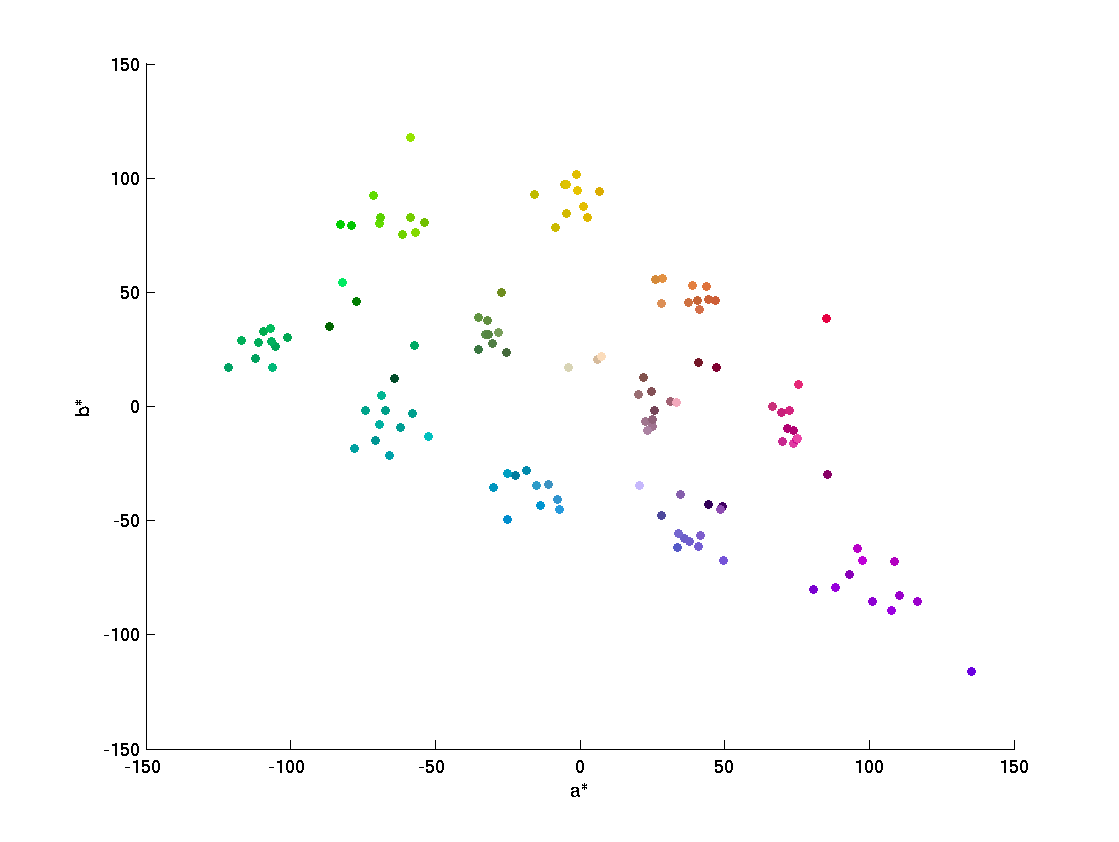
\includegraphics[width=.47\textwidth]{./experiments/figures/categories-language.pdf}
  \label{f:language-categories-language}
}
\subfigure[]{
    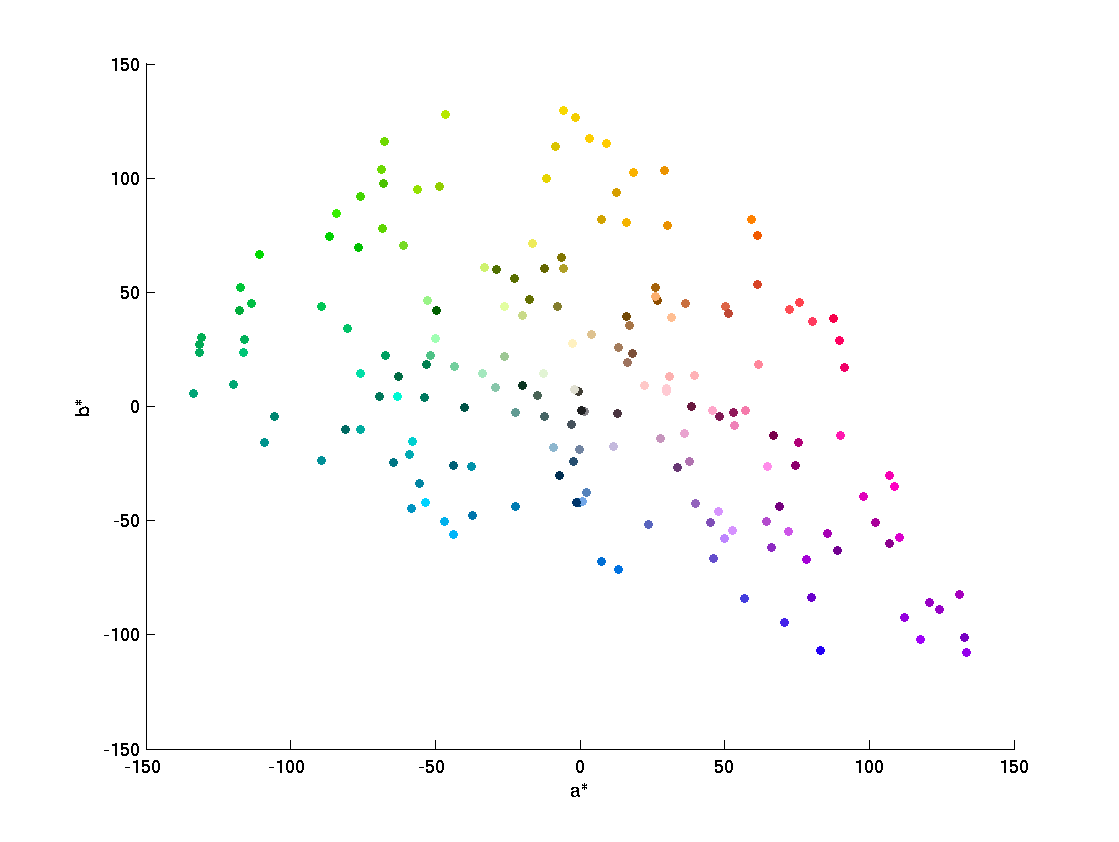
\includegraphics[width=.47\textwidth]{./experiments/figures/categories-no-language.pdf}
  \label{f:language-categories-no-language}
}
\caption[Resulting categories of all agents in a population in a
formation experiment and a discrimination experiment]{Resulting
  categories of \subref{f:language-categories-language} all agents in
  a population of 10 agents at the end of a formation experiment and
  \subref{f:language-categories-no-language} 10 agents learning
  categories individually in a discrimination experiment.}
\label{f:language-categories}
\end{figure}

\subsection{Alignment over different populations}

In their groundbreaking research, \cite{berlin69basic} studied
colour naming of 20 different languages around the world, which showed
remarkable cross-cultural similarities. Some colour samples from the
Munsell chart seemed to be more likely to become named by a colour
term than others which moreover correspond to the 11 basic colour
terms in English. This study received heavy criticisms, such as
eliciting information only from a very low number of informants. Most
of these criticisms have been addressed in a follow-up study, which
studied pre-industrial 110 languages \citep{kay10world}. The resulting
typology of these 110 languages are shown in a contour plot over the
histogram of the Munsell chart in Figure \ref{f:contour-wcs}. Some
regions in the chart are more likely to become the foci that are named
in a language. These regions are claimed to correspond to the English
colour foci. Analysis of the resulting data has confirmed the
existence of universal trends \citep{regier05focal}. These results are
however still controversial (see for example \cite{roberson02color,
  roberson05color}).

\begin{figure}[htbp]
\centering
  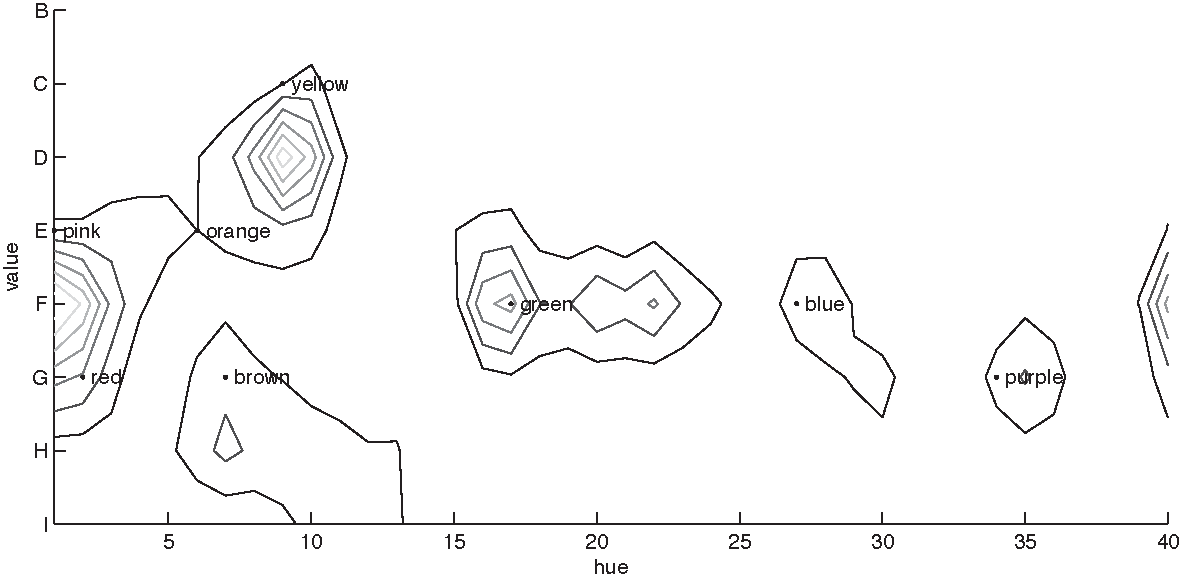
\includegraphics[width=.85\textwidth]{./experiments/figures/contour-wcs}
  \caption[Contour plot of the World Colour Survey]{Contour plot of
    the histogram of foci over the Munsell diagram for the 110
    languages studied in the World Colour Survey. The lighter the
    contour lines, the higher the histogram. The foci of the colour
    categories for English are shown for reference.}
\label{f:contour-wcs}
\end{figure}

One of the main questions is whether the proposed implementation of
the \emph{basic colour strategy} in which the focus is put on the
linguistic/cultural constraints, is capable of reproducing such
trends. If culture is largely arbitrary, then colour categories are
expected to be largely arbitrary as well \citep{roberson05color}. Two
separate populations will end up with different colour categories,
even if these populations start out under the same conditions.

I compare two experiments: a discrimination experiment, in which
language has no impact on the formation of the colour category system,
and a formation experiment, in which language does apply some pressure
to the formation process. Each experiment is run 105 times in a
population of 10 agents in two different environmental conditions: one
is based on the natural data set and the other one on the uniform data
set (Section \ref{s:simulated-data-sets}). The context consists of
three colour samples and the minimal distance between the different
samples in the context varies between 40 and 60 (5 runs for each
integer increment) in the CIE $L^*a^*b^*$ colour space.

The resulting categories of the different runs are collected and
presented as a contour plot of the histograms on the Munsell diagram
in Figures
\ref{f:contour-natural-no-language}-\ref{f:contour-uniform-language}.
Interestingly, the histograms that are produced by the experiments are
not flat but contain some structure.

\begin{figure}[htbp]
\centering
  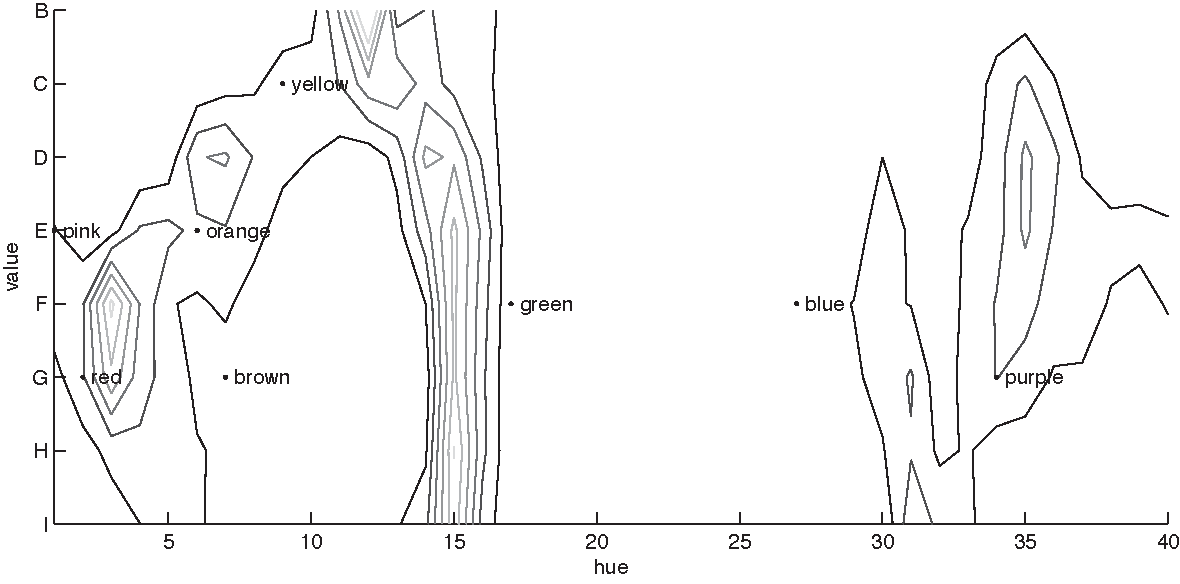
\includegraphics[width=.85\textwidth]{./experiments/figures/contour-natural-no-language}
  \caption{Contour plot of the resulting categories of 105 runs of the
    discrimination experiment using the natural data set.}
\label{f:contour-natural-no-language}
\end{figure}

\begin{figure}[htbp]
\centering
  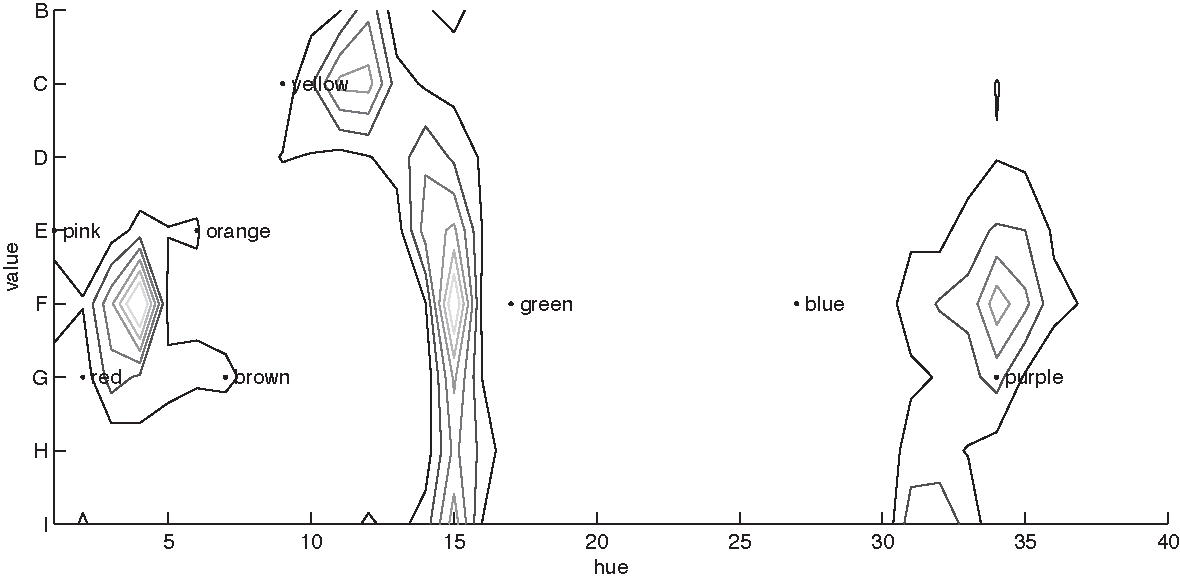
\includegraphics[width=.85\textwidth]{./experiments/figures/contour-natural-language}
  \caption{Contour plot of the resulting categories of 105 runs of the
    formation experiment using the natural data set.}
\label{f:contour-natural-language}
\end{figure}

\begin{figure}[htbp]
\centering
  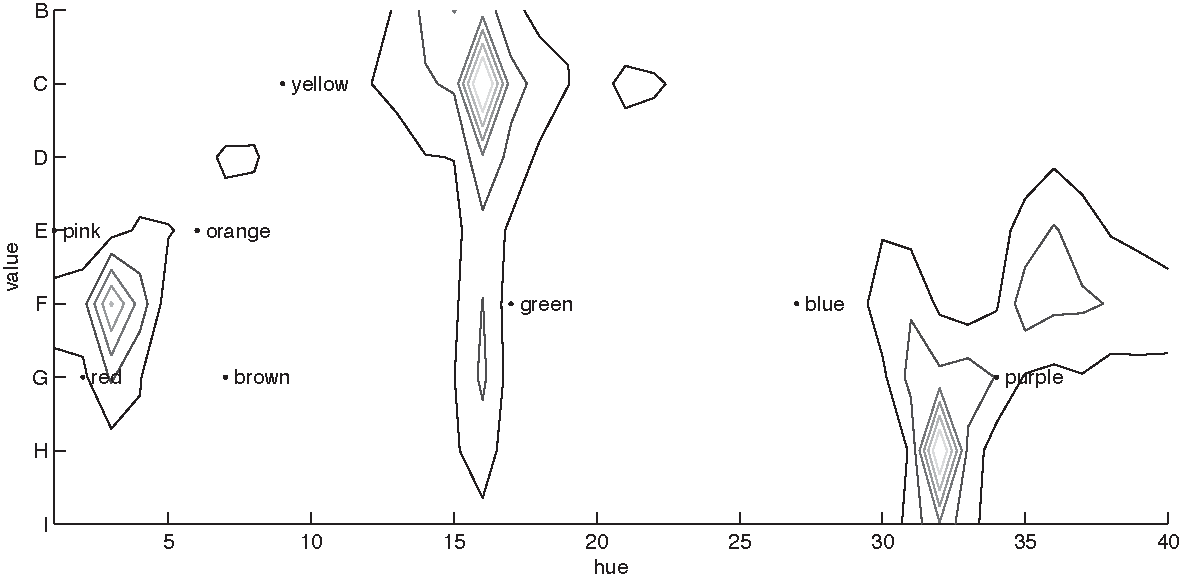
\includegraphics[width=.85\textwidth]{./experiments/figures/contour-uniform-no-language}
  \caption{Contour plot of the resulting categories of 105 runs of the
    discrimination experiment using the uniform data set.}
\label{f:contour-uniform-no-language}
\end{figure}

\begin{figure}[htbp]
\centering
  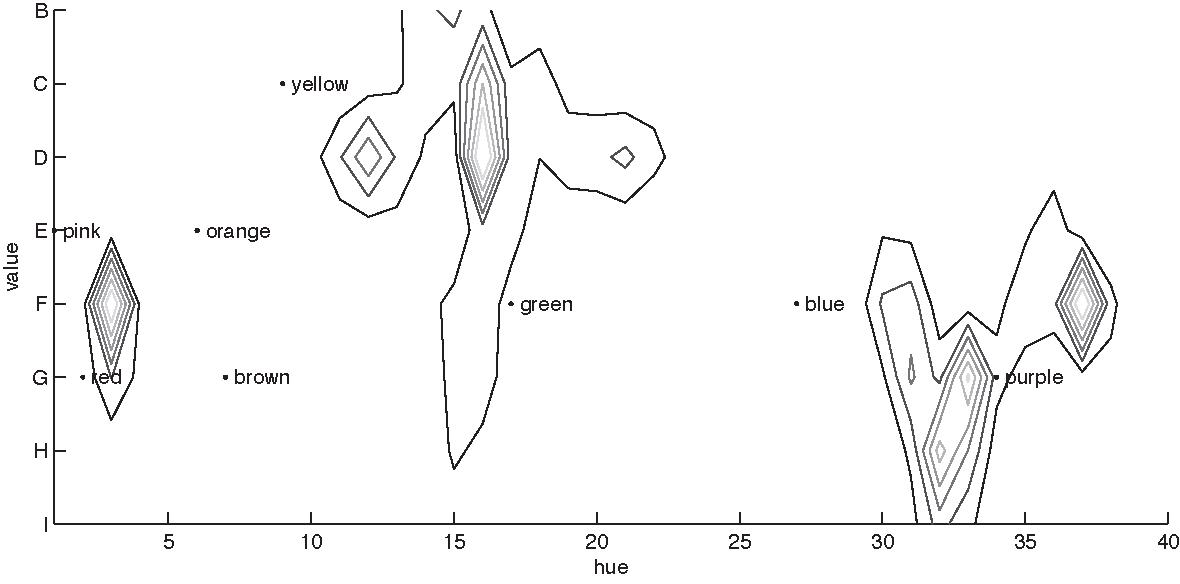
\includegraphics[width=.85\textwidth]{./experiments/figures/contour-uniform-language}
  \caption{Contour plot of the resulting categories of 105 runs of the
    formation experiment using the uniform data set.}
\label{f:contour-uniform-language}
\end{figure}

To compare the simulation results with the data from the World Color
Survey, I first determine the location of the highest peaks in all
histograms. This is done by a search for local maxima in the
histogram. Local maxima are connected components of histogram values
with the same value \emph{v}, whose external boundaries all have a
value less than \emph{v}. Next I compare the 10 highest peaks of the
World Color Survey data with the 10 highest peaks of our simulation
data. This is done by computing the undirected Hausdorff distance
\citep{rucklidge97efficiently}. The undirected Hausdorff distance
$H(A, B)$ between two sets of coordinates $A$ and $B$ is computed as
in Equations \ref{e:hausdorff-1}-\ref{e:hausdorff-2}, with $d(s, t)$
being the Euclidean distance between coordinates $s$ and $t$.

\begin{align}
H(A, B)& = \max (h(A,B), h(B,A)) 
\label{e:hausdorff-1} \\
h(S, T)& = \max_{s \in S} \left(\min_{t \in T} \left(d\left(s, t\right)\right)\right)
\label{e:hausdorff-2}
\end{align}

Figure \ref{t:comparison-to-wcs} shows the distance between the
highest WCS peaks and the highest peaks of the simulation results. The
best result is obtained when communicative constraints are present but
the environmental constraints are absent. This suggests that
environmental constraints are more of a burden than a blessing:
if the agents are allowed to sample the whole colour gamut, they form
categories at locations that are more closely to human colour
categories.

\begin{table}[htbp]
\centering
\begin{tabular}{ld{3}}
\lsptoprule
\emph{x} & \multicolumn{1}{c}{\emph{H(x, WCS)}} \\
\midrule
discrimination experiment, uniform data set & 5.39 \\
discrimination experiment, natural data set & 7.00 \\
formation experiment, uniform data set & 5.10 \\
formation experiment, natural data set & 7.00\\
\lspbottomrule
\end{tabular}
\caption[Distance between resulting topologies and WCS data]{Hausdorff
  distance between resulting topologies and WCS data. The lower the
  distance, the more similar to the WCS data.}
\label{t:comparison-to-wcs}
\end{table}

\subsection{Conclusion}

I have shown the coordinating role of language which allows agents to
align their colour categories. When no linguisic or cultural feedback
mechanism is in place, the colour categories of the agents are spread
out over the complete conceptual space. The impact of language on the
alignment over different populations is less pronounced: although some
universal trends seem to pop up, the additional effect of language
seems rather limited. I have been able to show that environmental
constraints are more of a curse than of a blessing if one wants to
explain the universal trends that exist in human colour category
systems around the world. Other constraints,  for example the
structure of the internal conceptual space or properties of the
classification algorithm, most likely play a bigger part to explain
these trends.

\section{Impact of embodiment on performance of operators}
\label{s:experiments-grounded}
\is{impact!of embodiment on basic colour strategy}
\is{embodiment!impact of|see{impact}}

Most of the previous studies on the formation and coordination of
colour category systems have assumed that no difference exists in how
interacting agents perceive the colour stimuli in the context. This is
not very realistic for embodied interactions in which agents perceive
colourful objects around them, using their own vision system. Embodied
agents will never share the same position in the world and hence will
perceive the objects from their own perspective. The colours of the
objects perceived by the agents will never be identical, due to for
example differences in lighting conditions or appearances when
perceived from different angles.

To investigate the influence of this \emph{perceptual deviation}, I
introduce the \emph{grounded colour naming game} in which agents are
embodied in humanoid robots (Figure
\ref{f:grounded-colour-naming-game}) and individually perceive scenes
through their cameras. The setup is similar to other language game
experiments with robots (e.g. Lego robots \citep{vogt03anchoring},
pan-tilt cameras \citep{steels98origins}, Sony Aibo robots
\citep{steels09perspective, loetzsch08typological} and the Sony
humanoid robots which are also used in this experiment
\citep{wellens08flexible}).

\begin{figure}[htpb]
  \centerline{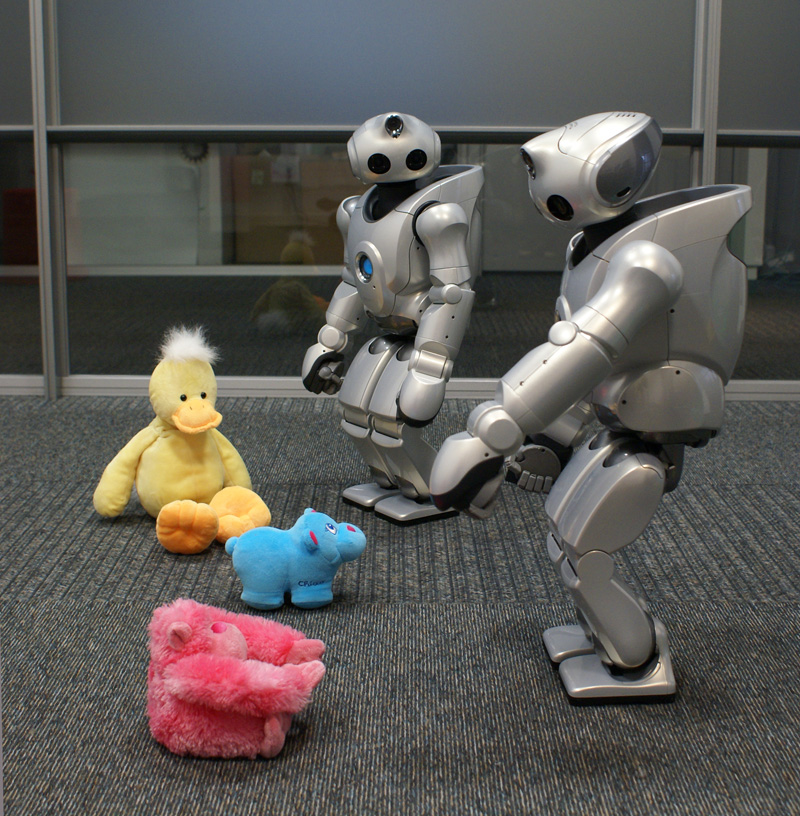
\includegraphics[width=0.65\textwidth]{./experiments/figures/grounding-cng-small}}
  \caption[The Grounded Colour Naming Game]{The \emph{Grounded Colour
      Naming Game}. It is similar to the \emph{Colour Naming Game} but
    involves embodied agents that perceive the world through their own
    vision system.}
\label{f:grounded-colour-naming-game}
\end{figure}

The embodied data used in this experiment was recorded by Michael
Spranger and Martin Loetzsch. Michael Spranger also developed the
vision system that is used by these robots.

\subsection{Robotic setup and visual perception}

The Sony humanoid robots \citep{fujita03autonomous} used in this
experiment are about 60 cm high, weigh approximately 7 kg and have 38
degrees of freedom. The robots are placed in a closed office
environment in which a set of coloured objects are placed. Before each
interaction, the experimenter modifies the current scene by adding or
removing an object or by changing the position or orientation of an
object in the scene. Each scene contains between two and four coloured
objects from a set of 20 objects (Figure \ref{f:object-sets}). The
main sensor used for perception is one of the three CCD cameras in the
head of the robot.

\begin{figure}[htbp]
  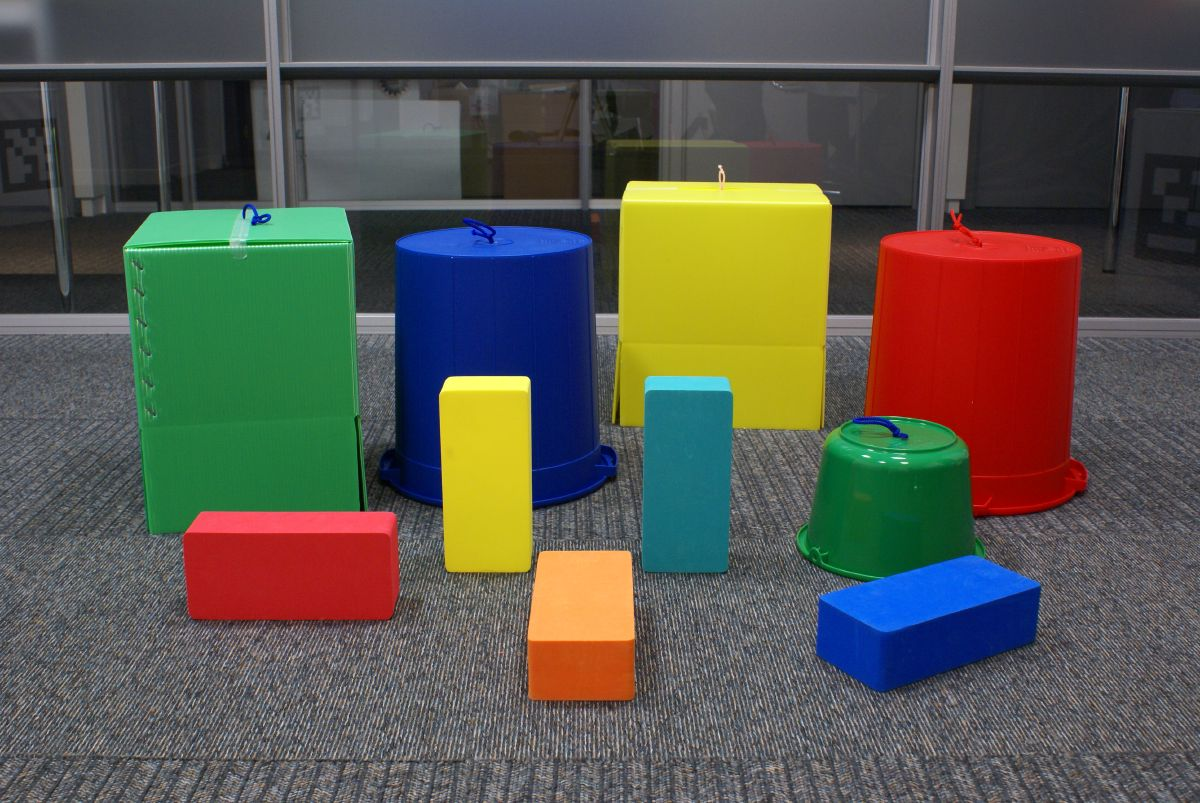
\includegraphics[width=0.47\textwidth]{./experiments/figures/grounding-data-sets-geometric-objects}
  \hspace{0.04\columnwidth}
  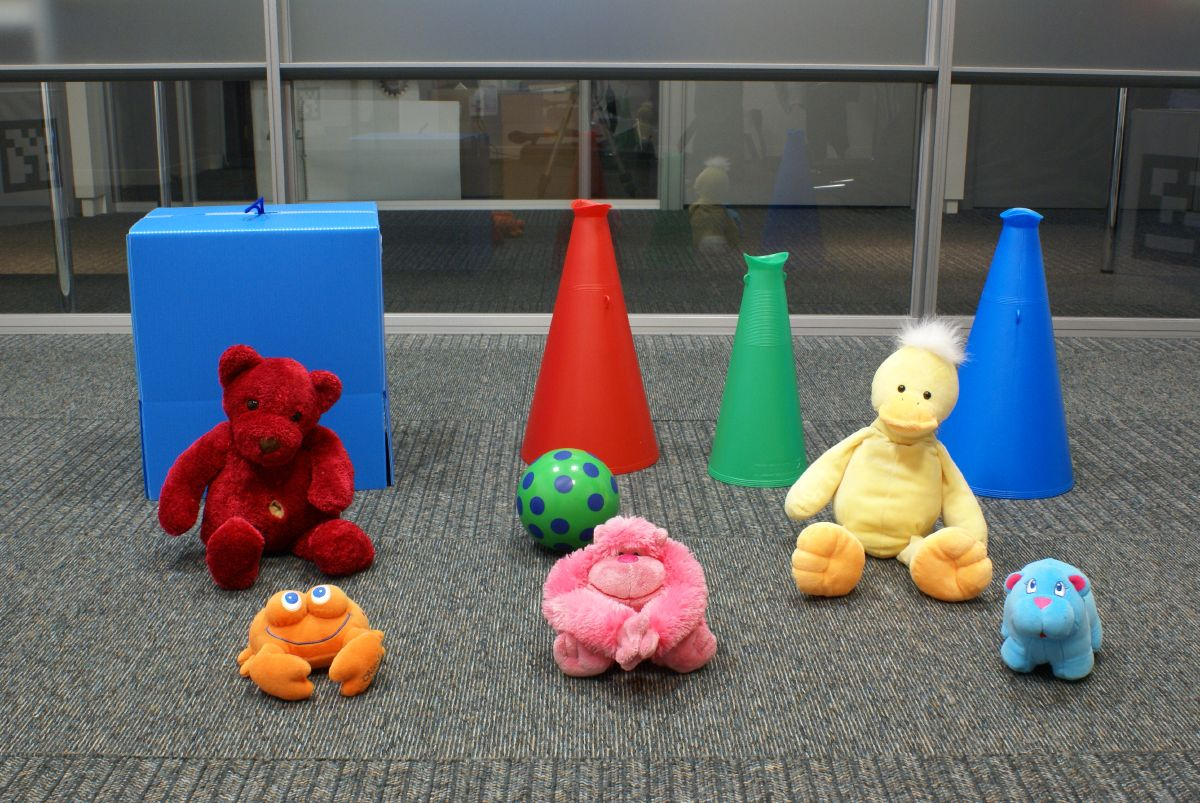
\includegraphics[width=0.47\textwidth]{./experiments/figures/grounding-data-sets-toy-objects}
  \caption[Objects that were represented to the robots]{Objects that
    were presented to the robots. Left: ten geometric objects (carton
    boxes, buckets, foam bricks). Right: ten toy-like objects (cones,
    a ball, animals).}
  \label{f:object-sets}
\end{figure}

The main goal of the robot's vision system is to construct persistent
internal representations of the objects in the robot's
environment. This system involves three sub-systems. First,
low-level vision routines process raw camera images to yield basic
\emph{percepts} (Figures
\ref{f:perception-a}-\ref{f:perception-d}). Percepts are connected
regions that differ from the background of the environment. The
statistics of the environment's background are acquired in a
calibration phase.

\begin{figure}[htbp]
  \centering
  \subfigure[]{
    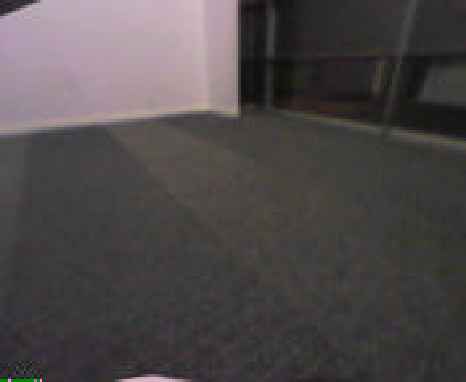
\includegraphics[width=0.3\columnwidth]{./experiments/figures/grounding-vision-system-object-perception-1}
    \label{f:perception-a}
  }
  \subfigure[]{	
    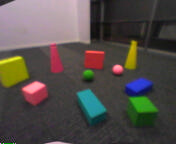
\includegraphics[width=0.3\columnwidth]{./experiments/figures/grounding-vision-system-object-perception-2}
    \label{f:perception-b}
  }
  \subfigure[]{	
    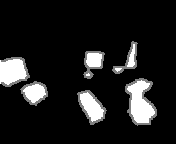
\includegraphics[width=0.3\columnwidth]{./experiments/figures/grounding-vision-system-object-perception-4}
    \label{f:perception-c}
  }
  \subfigure[]{	
    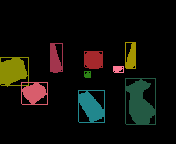
\includegraphics[width=0.3\columnwidth]{./experiments/figures/grounding-vision-system-object-perception-5}
    \label{f:perception-d}
  }
  \subfigure[]{	
    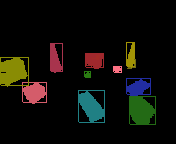
\includegraphics[width=0.3\columnwidth]{./experiments/figures/grounding-vision-system-object-perception-7}
    \label{f:perception-e}
  }\subfigure[]{
    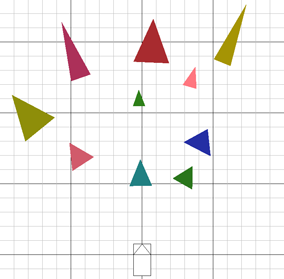
\includegraphics[width=0.3\columnwidth]{./experiments/figures/grounding-vision-system-object-modeling-2}
    \label{f:perception-f}
  }
  \caption[The object vision system]{The object vision
    system. \subref{f:perception-a}: a raw camera image taken during
    the calibration phase. \subref{f:perception-b}: a camera image of
    a scene containing objects. \subref{f:perception-c}: the result of
    noise-reduced foreground/ background
    classification. \subref{f:perception-d}: the segmented foreground
    regions drawn in their average colour and with bounding
    boxes. Note that the partially overlapping blue and green blocks
    in the right bottom of the original image are segmented into the
    same foreground region. \subref{f:perception-e}: classification of
    foreground pixels using existing colour models. Pixels are drawn
    in the average colour of the most similar object
    model. \subref{f:perception-f}: computation of colour, position
    and size in a robot-egocentric reference system. The width and
    height of objects is indicated by the width and height of the
    triangles.}
  \label{f:object-perception}
\end{figure}

Second, these foreground regions are tracked in subsequent camera
images despite changing positions and appearances of the objects. In
order to do so, the vision system needs to establish a correspondence
between the internal \emph{object model} and the image regions that
refer to the same physical object, a process known in robotics as
\emph{anchoring} \citep{coradeschi03anchoring}. Colour histograms of
already established object models are used to classify image regions
with respect to their similarity to object models (Figure
\ref{f:perception-d}). Kalman Filters \citep{kalman60new} are used to
associate classified regions to object models based on colour
similarity and position in the image (Figure \ref{f:perception-e}).

Third, when needed in communicative interactions, the vision system
encodes a set of visual properties about each object model. These
properties are colour, position, height and width, but in this
experiment only the colour information of each object is used. The
camera of the robot delivers up to 30 images per second with a
resolution of 176$\times$144 pixels in the YCrCb colour space. The
colour of the object is the average colour of all pixels that make up
the object. This average colour is transformed into the perceptually
equidistant colour space CIE \emph{L*a*b*} (using the equations
described in Appendix \ref{s:spaces}). Furthermore, in order to be able
to point to objects, the position of objects is computed in a robot
egocentric reference system (Figure \ref{f:perception-f}).

The robotic setup, including the vision system and mechanisms to
establish \emph{joint attention} \citep{tomasello95jointattention}, is
described in more detail in other background papers
\citep{spranger08diplomathesis, loetzsch10grounding}.

\subsection{Perceptual deviation and structure in embodied data}
\label{s:embodied-data}

When moving from simulated to embodied experiments, the colour stimuli
differ in two main ways. The first difference is that in embodied
experiments, it is very unlikely that both speaker and hearer
experience the colours of a physical object in an identical way as
lighting conditions and appearances of objects may vary from the
different perspectives of the robots. This is what I call
\emph{perceptual deviation}, which is illustrated in Figure
\ref{f:scene-example}. The average difference in perceptual
experiences for the same objects in the world across all scenes used
in our experiment, is shown in Figure \ref{f:perceptual-deviation}.

\begin{figure}[htbp]
  \centering%\small
  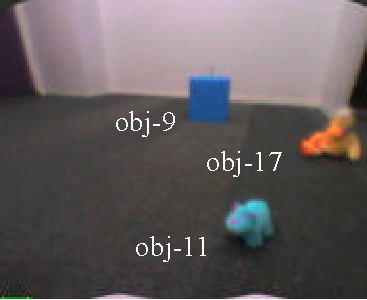
\includegraphics[width=0.37\textwidth]{./experiments/figures/grounding-scene-a}
  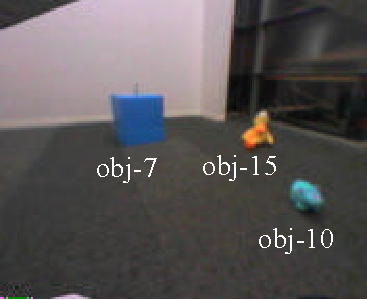
\includegraphics[width=0.37\textwidth]{./experiments/figures/grounding-scene-b}
  \begin{tabularx}{.75\textwidth}{l *{6}{d{2}}}
%     & \multicolumn{3}{c}{}
%     & \multicolumn{3}{c}{} \\
  \lsptoprule
    & \multicolumn{1}{c}{obj-9} & \multicolumn{1}{c}{obj-11} & \multicolumn{1}{c}{obj-17} & \multicolumn{1}{c}{obj-7} & \multicolumn{1}{c}{obj-15} & \multicolumn{1}{c}{obj-10} \\
    \midrule
    \emph{L*} & 35.5 & 51.2 & 50.5 & 35.6 & 62.2 & 52.8  \\
    \emph{a*} & 7.7 & -17.1 & 26.7 & 7.2 & 27.9 & -20.1   \\
    \emph{b*} & -40.7 & -14.0 & 39.6 & -39.0 & 52.5 & -11.3  \\
    \lspbottomrule
  \end{tabularx}
  \caption[Comparison between the colour perceptions of two robots for
  an example scene]{Comparison between the colour perceptions of two
    robots for an example scene. The robots see the yellow duck
    (obj-17 for the left robot and obj-15 for the right robot) from
    different sides and distances and thus perceive very different
    \emph{a*} and \emph{b*} values for the same object.}
  \label{f:scene-example}
\end{figure}

\begin{figure}[htbp]
\begin{center}
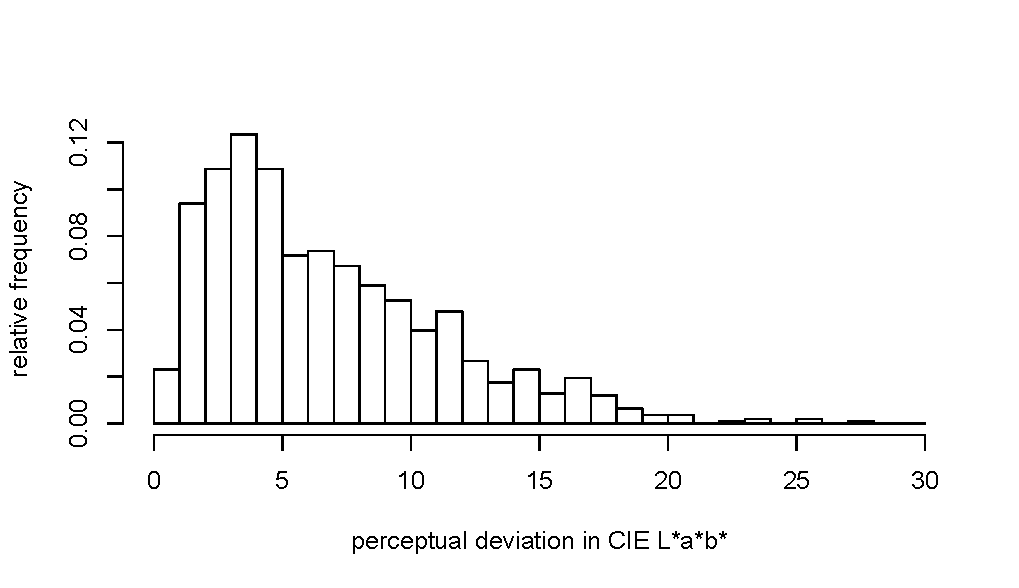
\includegraphics[width=.9\textwidth]{./experiments/figures/grounding-perceptual-deviation.pdf}
\caption[Perceptual deviation between the speaker and the hearer]{A
  histogram of the perceptual deviation between the speaker and the
  hearer for the grounded data set used for the experiments reported
  in this paper (mean = 6.721; st. dev. = 4.575). This distribution is
  skewed towards lower deviations.}
\label{f:perceptual-deviation}
\end{center}
\end{figure}

The second main difference between simulated stimuli and embodied data
is that the colour stimuli in embodied experiments contain a higher
level of \emph{structure}. Because the number of used objects is
typically limited in embodied experiments due to practical constraints
(in our experiment to 20 objects), some colours do not occur at all
while other colours will appear more often than others (Figure
\ref{fig:grounded-world}). Using a one nearest-neighbour
classification algorithm, I determine the relative frequency of the
English colour categories \citep{sturges95location} in the grounded
data: red (.28), green (.20), purple (.12), black (.11), blue (.10),
brown (.09), orange (.04) and yellow (.04). The colour categories
pink, grey and white are not represented in the grounded data.

\begin{figure}[htbp]
\begin{center}
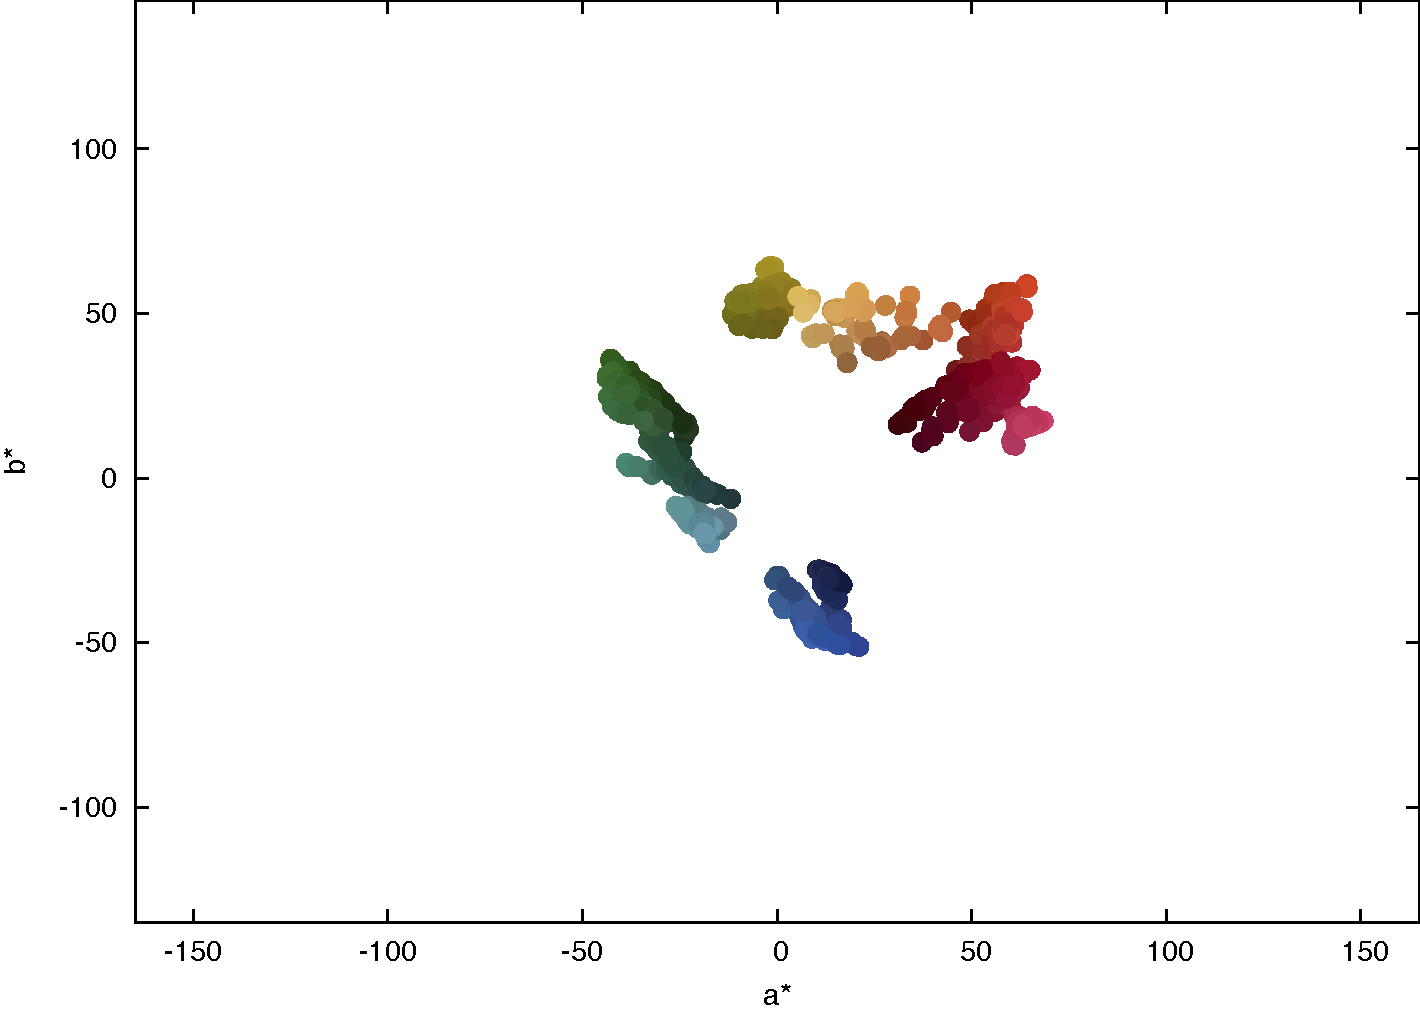
\includegraphics[width=\textwidth]{./experiments/figures/grounding-grounded-world.pdf}
\caption[Structure of the grounded data set]{The colours of all the
  objects in all contexts in the dataset used in our experiment
  projected on the hue plane of the CIE \emph{L*a*b*} colour
  space. The colour data in the embodied experiment is clearly
  structured, with more colours appearing around the actual colour of
  the objects used.}
\label{fig:grounded-world}
\end{center}
\end{figure}

In contrast, artificially generated contexts usually consist of a
(constrained) subset of a larger set of stimuli, like for example the
set of all Munsell chips within the visual spectrum (Figure
\ref{f:munsell}) which was originally used in anthropological research
\citep{kay10world, maclaury97color}. Such a set possibly reflects the
colour distributions of real-world environments based on a series of
photographs, such as an urban or natural environment (see Section
\ref{s:impact-of-environment}). If no such distribution is reflected,
such as for example in the set of Munsell chips, each stimulus will as
likely be represented in a shared context. Although stimuli sets that
do reflect real-world colour distributions contain more structure than
those that do not, the embodied data set is far more structured, as it
reflects the different appearances of a limited number of objects.

\subsection{Discerning the impact of embodiment}

I compare three environmental conditions to discern the influence of
the two main differences when moving from simulated to real-world
perception. In the first condition (shared simulated perception),
agents will perceive artificial contexts which are sets of randomly
chosen Munsell chips. In the second (shared grounded perception), both
agents artificially share the same grounded perception coming from one
robot body. In the third (individual grounded perception), both agents
perceive the environment through their individual robot bodies.

In order to measure the influence of the structure in a grounded
world, I compare the performance of conditions I and II. Basic
characteristics of the scenes in condition II are carefully controlled
in condition I. These characteristics are based on the set of all
embodied scenes used and entail the distribution of context sizes, the
total number of colour stimuli and the minimal and maximal distance
between different colours within one scene/context. The better these
characteristics are controlled, the better I can discern the impact of
the structure in the embodied data.

To quantify the impact of the perceptual deviation between speaker and
hearer, I compare conditions II and III.

\subsection{Resulting dynamics}

The three environmental conditions are compared across four different
experiments. The first baseline experiment is similar to the one
introduced earlier (Section \ref{s:basic-baseline-experiment}) except
that now the predefined language system is based on the English
category system \citep{sturges95location}. This experiment gives an
idea about how two English human subjects would perform in the three
different environmental conditions. The resulting communicative
success is shown in Figure \ref{f:comparison-communicative-success},
which is roughly around 80\%. The interactions in which the two agents
fail, are those in which the topic could not be discriminated. The
presence of structure in the world has a positive impact on
communicative success and the additional problem posed by perceptual
deviation seems to have negative impact. This negative impact is
rather limited, which resonates with a previous analysis of the same
grounded data which indicated that colour is the least variable when
different perspectives are used, unlike for example the spatial
positions of the objects \citep{wellens08flexible}.

\begin{figure}[htbp]
\begin{center}
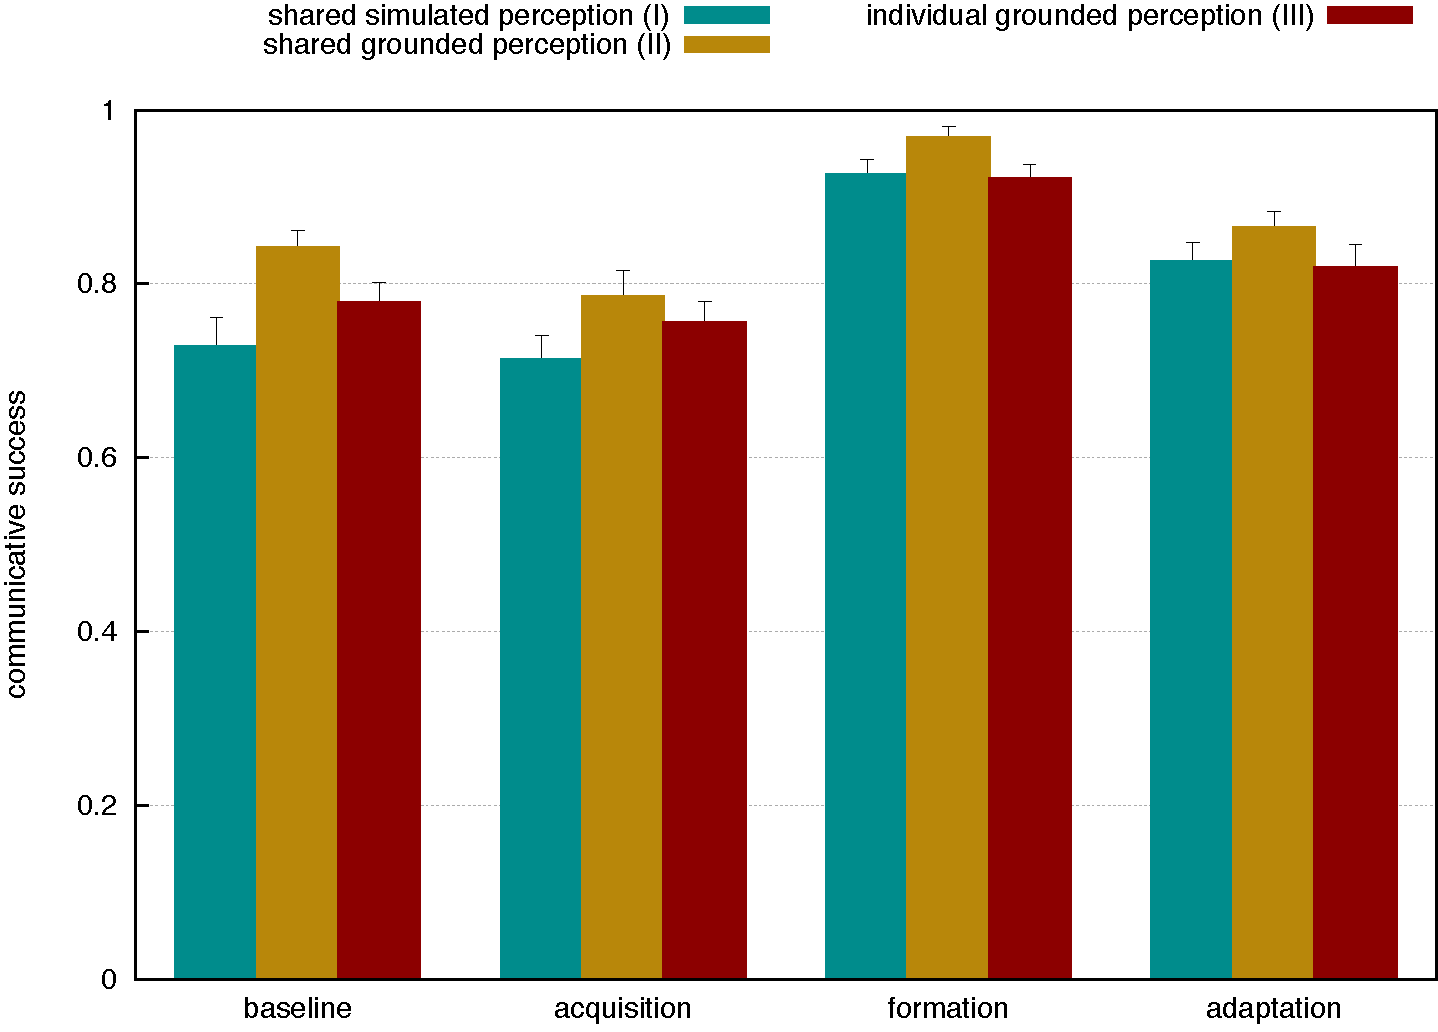
\includegraphics[width=0.9\textwidth]{./experiments/figures/grounding-comparison-communicative-success.pdf}
\caption[Communicative success in three different conditions for four
types of experiments]{Resulting communicative success of four
  different experiment types for the three different conditions,
  grouped per experiment type. The predefined language system is based
  on the English colour category system. The results are shown after
  2k games for the acquisition experiment and after 10k games/agent in
  the formation and the adaptation experiment. The results are
  averaged over 10 runs.}
\label{f:comparison-communicative-success}
\end{center}
\end{figure}

In the acquisition experiment, one agent needs to master the English
colour lexicon from another agent using the adoption and alignment
operators introduced in Section
\ref{s:bcs-adoption-alignment-operators}. These operators result in a
level of communicative success that is almost as high as in the
baseline experiment after 2k games using the 8 colour terms for the
colour categories that are represented in the grounded data (see
Section \ref{s:embodied-data}). This indicates that the used operators
are adequate to acquire an ontology from another agent.

Figure \ref{f:comparison-communicative-success} shows the
communicative success in a formation experiment for a population of 10
agents after 10k games per agent. These agents are more successful
than the ones in the baseline and acquisition experiment, mainly due
to the higher number of colour categories (around 20 for conditions II
and III and 25 for condition I). Figure
\ref{f:formation-interpretation-variance} shows the interpretation
variance (the average distance between the prototypes of the colour
categories associated with the same form within the population) of the
population over time. It is significantly lower for conditions II and
III because the structure in the environment restricts the possible
location of the colour categories used by the agents. It is also
slightly lower when both agents share their perception.

\begin{figure}[htbp]
\begin{center}
  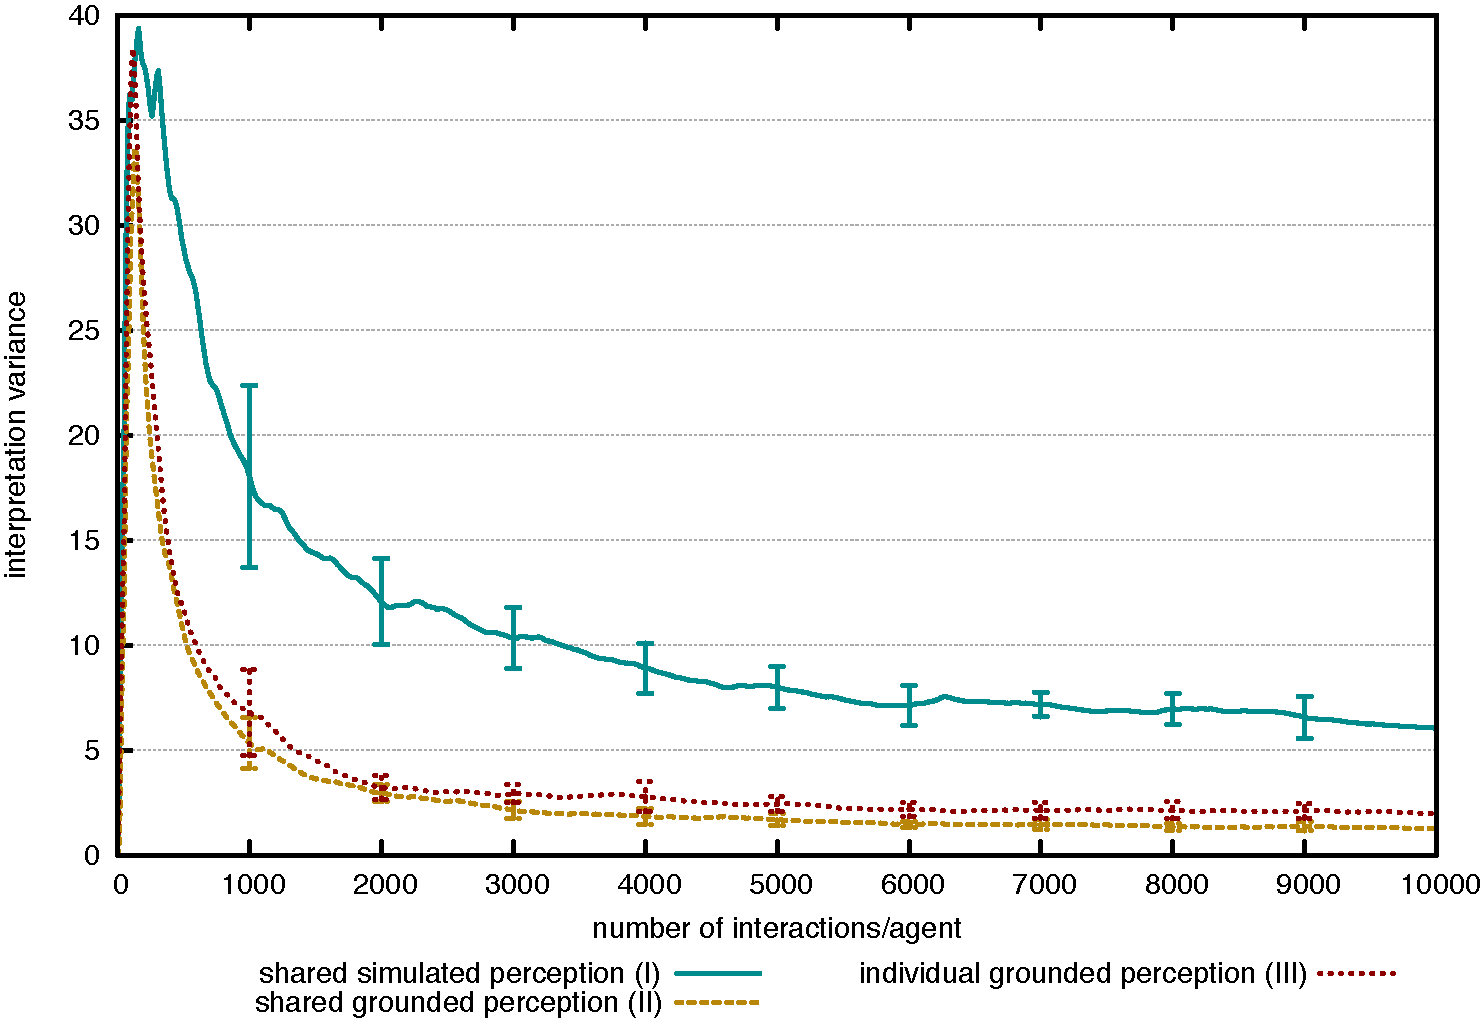
\includegraphics[width=.9\textwidth]{./experiments/figures/grounding-formation-interpretation-variance.pdf}
  \caption[Interpretation variance in grounded formation experiment in
  three experimental conditions]{The interpretation variance in
    formation experiments is significantly lower for the grounded
    conditions than for shared simulated perception. In the grounded
    condition it is lower when perception is shared between both
    interacting agents.}
\label{f:formation-interpretation-variance}
\end{center}
\end{figure}

Finally, I have studied the impact of having adaptive colour
categories, independent of the ontology size, in an adaptation
experiment. In this experiment a population of 10 agents starts out
with a colour lexicon based on the English colour categories but is
allowed to change these categories to its functional needs using the
alignment operator. The invention and adoption operators are
disabled. The communicative success after 10k games per agent is shown
in Figure \ref{f:comparison-communicative-success}. Compared to the
success of the baseline experiment, an overall improvement is observed
in all three conditions.

\subsection{Comparison to human categories}

I compare the resulting ontologies to the colour categories of English
\citep{sturges95location} using two different methods: the direct
comparison method and a naming benchmark. In the direct
comparison method, I compute the distance between the two ontologies
in the CIE \emph{L*a*b*} colour space. The lower this distance, the
more similar the two ontologies are. The naming benchmark consists of
naming the colour chips that were consistently named by English
subjects \citep{sturges95location} (shown in Figure
\ref{f:basic-consensus-chips-english}). The higher the performance on
this benchmark, the more similar the performance of the agents to
human performance is. Both methods require a matching procedure in
which each category of the resulting ontology is paired to a category
of the English ontology in such a way that the pair-wise distance in
the colour space is minimal.

Using these two methods, I compare the ontologies resulting from two
different experiment types: the acquisition experiment and the
formation experiment. To rule out the impact of ontology size on the
comparison, I control the maximum number of colour categories in the
formation experiment to be the number of categories that are learned
in the acquisition experiment. As in the acquisition experiment, the
teacher only uses the colour terms that are present in the embodied
dataset, which are listed in Section \ref{s:embodied-data}. This
maximum number of colour categories is set to 8. For each experiment
type, I compare the three environmental conditions as described in the
previous section.

The results of the direct comparison method and the naming benchmark
are shown in Figure \ref{f:comparison-distance-to-human-categories}
and Table \ref{t:benchmark} respectively. Both methods show that in
general, the acquisition experiments lead to ontologies that are more
similar to the colour categories of English than the formation
experiment. The main reason for this is that in the acquisition
experiment the predefined colour lexicon of the speaker is identical
to the one I compare to and hence guides the learner to categories
that are similar to the English colour lexicon, whereas in the
formation experiment no such guidance is present.

\begin{figure}[htbp]
\begin{center}
  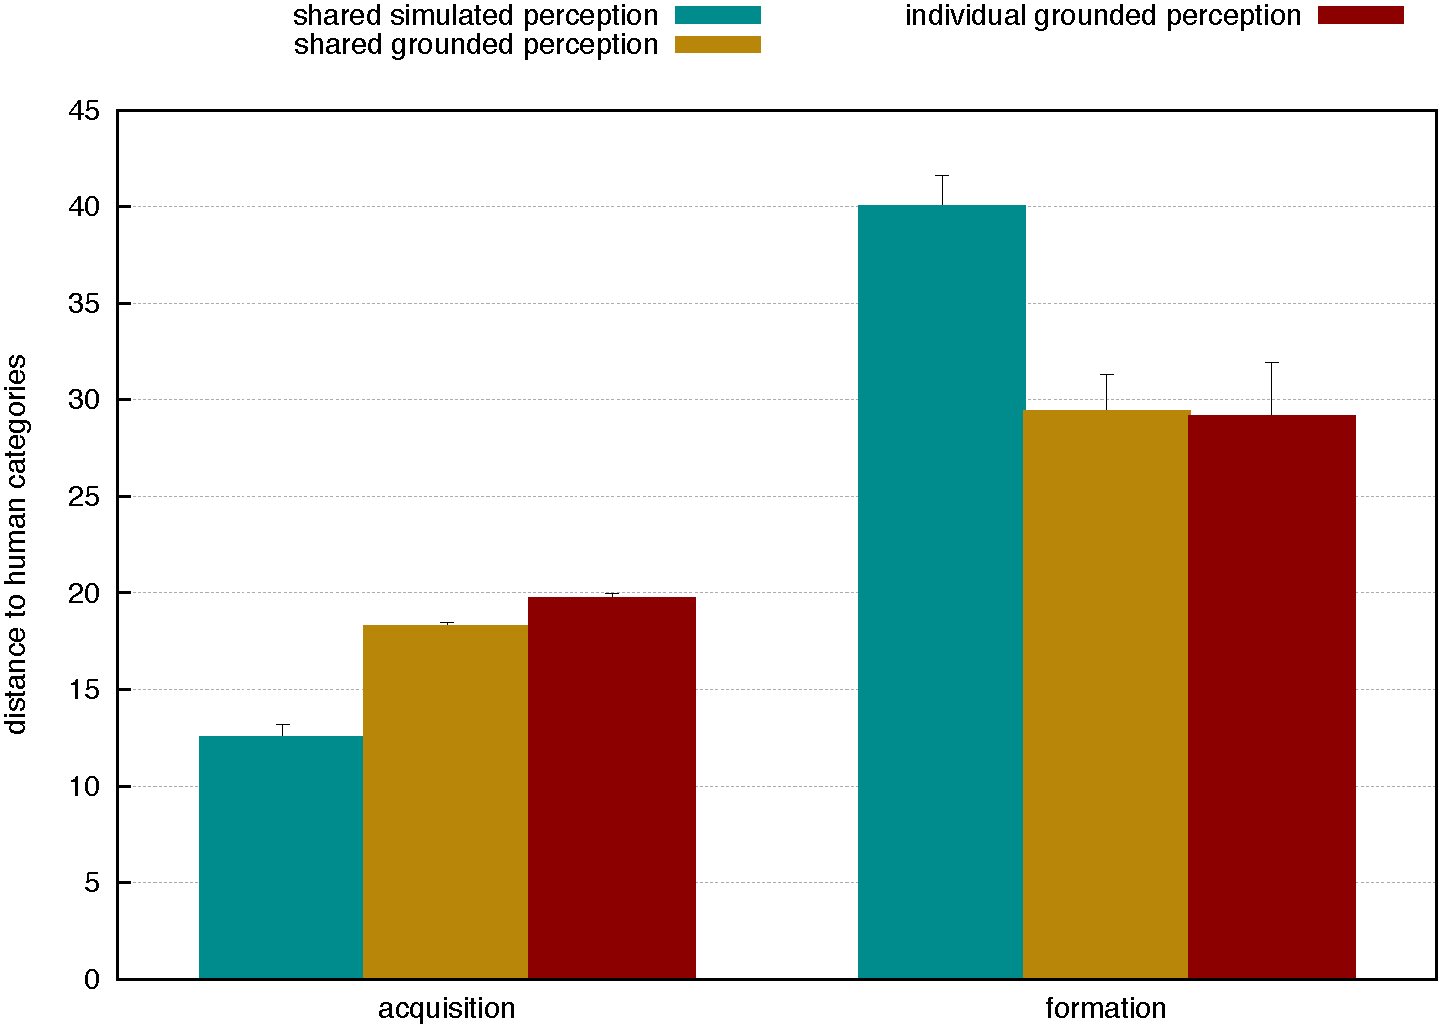
\includegraphics[width=0.9\textwidth]{./experiments/figures/grounding-comparison-distance-to-human-categories.pdf}
  \caption[Direct comparison between formed grounded colour category
  systems and the English colour categories]{Results of the direct
    comparison method. Two experiment types are compared in three
    environmental conditions, grouped per experiment type: the
    acquisition experiment (2k games) and the formation experiment
    (population of 10 agents; 10k games per agent). The results are
    averaged over 10 runs.}
\label{f:comparison-distance-to-human-categories}
\end{center}
\end{figure}

\begin{table}[htbp]
  \centering
  \begin{tabularx}{.85\textwidth}{l *{8}{d{2}}d{4}}
  \lsptoprule
    & \multicolumn{1}{X}{\centering RE} & \multicolumn{1}{X}{GN} & \multicolumn{1}{X}{\centering PU} & \multicolumn{1}{X}{\centering BK} & \multicolumn{1}{X}{\centering BL} & \multicolumn{1}{X}{\centering BR} & \multicolumn{1}{X}{\centering OR} & \multicolumn{1}{X}{\centering YL} & \multicolumn{1}{X}{\centering\scshape total} \\
    \midrule
    & 4 & 22 & 14 & 3 & 25 & 4 & 6 & 8 & 86 \\
    \midrule
    & 4 & 19 & 14 & 3 & 22 & 4 & 6 & 8 & 80 \\ 
    \midrule
    I & 4 & 15.7 & 10.3 & 3 & 21.8 & 3.7 & 6 & 8 & 72.5 \\
    II & 4 & 17.5 & 9.6 & 3 & 21.1 & 4 & 6 & 8 & 73.2 \\
    III & 4 & 16.5 & 10.2 & 3 & 21.7 & 4 & 6 & 8 & 73.4 \\
    \midrule
    I & 1.6 & 3 & 6.7 & 3 & 6.2 & 0 & 2.8 & 7.9 & 31.2 \\
    II & 1.9 & 14.3 & 10.5 & 1.1 & 10.3 & 0.1 & 3.5 & 7.6 & 49.3 \\
    III & 1.7 & 13.4 & 7.7 & 2 & 9.7 & 0.3 & 3.6 & 7.4 & 45.8 \\
    \lspbottomrule
  \end{tabularx}
  \caption[Naming benchmark of formed grounded colour category systems
  for the consensus chips in English]{Results of the naming benchmark,
    broken down by category: red (re), green (gn), purple (pu), black
    (bk), blue (bl), brown (br), orange (or) and yellow (yl).  The top
    part shows the baseline performance using the centroids of the
    English colour ontology. The middle and bottom part show the
    performance of the acquisition experiment, respectively formation
    experiment, for the three environmental conditions.}
  \label{t:benchmark}
\end{table}

In the acquisition experiment, condition I seems to yield ontologies
that are more similar to human colour categories than conditions II
and III, as shown in the results of the direct comparison method. The
prototypes of the categories acquired by the learner are situated on
the centre of all stimuli that the speaker has named using the term
that is associated with that category. In conditions II and III some
colour categories are only partially represented, and hence the
location of the prototypes acquired by the learner do not fully
correspond to the locations of the prototypes of the teacher. In
condition I however, all categories are fully represented, leading to
a smaller difference with the ontology of the teacher. The results of
the naming benchmark show no clear distinction between the three
environmental conditions for this experiment.

In the formation experiment, both comparison methods suggest that
conditions II and III produce ontologies that are more similar to
English colour categories than condition I. Although in this
experiment no guiding teacher is present, the structure in the
grounded data partially takes over the guiding role of the
teacher. The colours of the objects presented to the robots (Figure
\ref{f:object-sets}) are better examples of the basic colour
categories for English than the stimuli in the simulated world in
which no such structure is present.

\subsection{Conclusion}

I have shown that our model for the colour naming game is robust
enough to overcome the main difficulties arising from embodiment in an
experiment using humanoid robots. In embodied experiments, speaker and
hearer perceive the world from a different perspective and hence
experience the colours of the objects around them differently. In our
experimental setup, the impact of this perceptual deviation is rather
limited as the lighting conditions are constant in the office
environment.

I have attested the positive impact on the resulting communicative
success of adapting categories to the functional needs of the agents,
even when compared to an experiment in which static categories are
completely shared within a population. This finding resonates with
previous studies in experimental psychology
\citep{garrod94conversation}, in which it is shown that humans align
their ontologies when interacting with each other, even in the course
of a single dialogue.

As the resulting ontologies reflect the structure of the environment
in which they are developed, these ontologies will bear more
resemblance to the colour categories of English when the environment
consists of objects that are good examples of these categories than in
an environment in which the colours are uniformly distributed over the
colour spectrum.

\section{General conclusion}

I have accounted for a positive impact of the structure in the
environment on the similarity between simulated and natural language
systems, although part of this impact is accounted for by general
categorisation principles that are inherent to the algorithms used. I
have shown the coordinating role of language between language users in
one community. I have also studied the impact of language and
environment on the universal trends observed in language systems
around the world. The environmental constraints seem to have a
negative impact, whereas language seems to have a slightly positive
impact. Finally, I have shown the impact of embodiment on the
performance of the adoption, alignment and invention operators and
compared the resulting language systems to the English basic colour
language system.

\newpage
\thispagestyle{empty}